\section{Casi d'uso}
I casi d'uso seguenti emergono da un'attenta analisi degli \textit{Analisti} del gruppo \GroupName{} rivolta al capitolato e da un'approfondita discussione con il proponente Proponente{}. Gran parte dei casi d'uso sono stati dedotti grazie all'esperienza derivata dall'utilizzo di glossario{ActiveAdmin}, un progetto analogo a ProjectName{} basato su glossario{Ruby on Rails}.\
Ogni caso d'uso è identificato univocamente e in modo gerarchico tramite una codifica nella forma:

\begin{center}

\textit{UC[codice dell'ambito][codice univoco del padre],[codice progressivo del figlio]}

\end{center} 

dove il \textbf{codice dell'ambito} può assumere i seguenti valori:

\begin{itemize}

  \item \textbf{U} - ambito utente, che comprende sia l'utente normale che l'\textit{admin} di una applicazione generata da \ProjectName{};
  \item \textbf{S} - ambito sviluppatore.

\end{itemize}


\subsection{Ambito Utente}
\subsubsection{UCU - Operazioni ad alto livello} 
    \begin{center}
    \begin{figure}[H]
      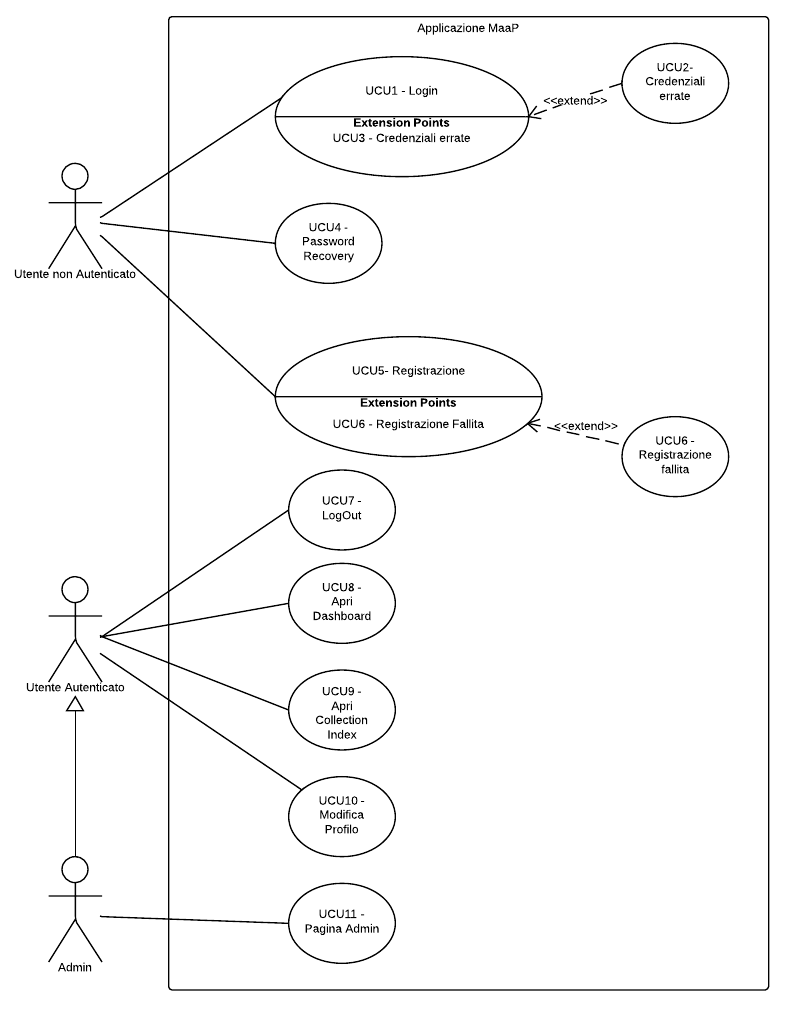
\includegraphics[scale=0.16]{UML/UCU - Operazioni ad alto livello.png}
      \caption{UCU - Operazioni ad alto livello} 
    \end{figure}
    \end{center}
    
      %Tabella 
      \begin{center}
      \bgroup
      \def\arraystretch{1.8}     
      \begin{longtable}{  p{3.5cm} | p{8cm} } 
            
      \hline
      \multicolumn{2}{ | c | }{ \cellcolor[gray]{0.9} \textbf{UCU - Operazioni ad alto livello}} \\ 
      \hline
      
      \textbf{Attori Primari} & Utente non autenticato, Utente autenticato, Admin \\ 
          \textbf{Scopo e Descrizione} & L'Utente non autenticato può autenticarsi inserendo le credenziali nell'apposito form e  recuperare le stesse qualora le abbia perse.
L'Utente autenticato in qualsiasi punto dell'applicazione può accedere alle seguenti funzionalità: accedere alla Dashboard, effettuare il Logout , può scegliere una qualsiasi collection presente e può modificare i propri dati. 
L'Utente Admin eredita le funzionalità dell'Utente Autenticato, può gestire gli utenti creandone di nuovi o modificandoli ed inoltre può gestire nuovi indici. \\ 
          
          \textbf{Precondizioni}  & L'applicazione Maap è funzionante e pronta all'utilizzo.\\ 
          
          \textbf{Postcondizioni} & L'applicazione ha ricevuto le informazioni sulle operazioni che l'utente vuole eseguire. \\
          
          \textbf{Flusso Principale} & 1. Utente non autenticato esegue il login (UCU1); 
2. Utente non autenticato può recuperare la password (UCU4);
3. Utente non autenticato può richiedere la registrazione (UCU5);
4. L'utente autenticato può decidere di effettuare il logout (UCU3);
5. L'utente autenticato può visualizzare la Dashboard (UCU8);
6. L'utente autenticato può scegliere una collection e visualizzarla (UCU9);
7. L'utente autenticato può scegliere di modificare i propri dati (UCU10);
8. L'admin può accede alla sua pagina di amministrazione per la gestione degli utenti (UCU11);
9. L'admin può gestire i possibili indici (UCU7).
 \\
           \textbf{Esclusioni} & 1.1. L'utente visualizza un errore dato dall'inserimento errato delle credenziali. (UCU2);
2.1. L'utente visualizza un errore dato dal fallimento della registrazione (UCU6). \\
      \end{longtable}
      \egroup
\end{center}

\subsubsection{UCU1 - Login} 
    \begin{center}
    \begin{figure}[H]
      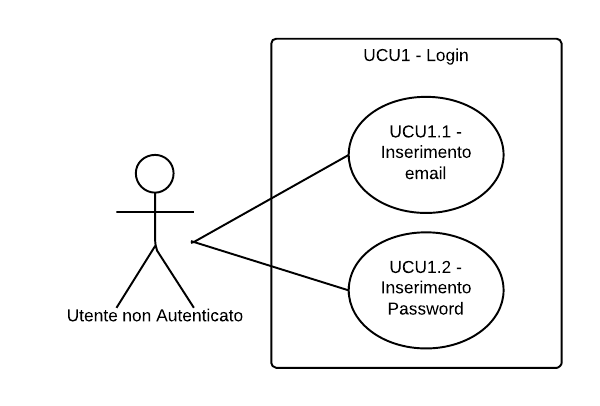
\includegraphics[scale=0.16]{UML/UCU1 - Login.png}
      \caption{UCU1 - Login} 
    \end{figure}
    \end{center}
    
      %Tabella 
      \begin{center}
      \bgroup
      \def\arraystretch{1.8}     
      \begin{longtable}{  p{3.5cm} | p{8cm} } 
            
      \hline
      \multicolumn{2}{ | c | }{ \cellcolor[gray]{0.9} \textbf{UCU1 - Login}} \\ 
      \hline
      
      \textbf{Attori Primari} & Utente non autenticato  \\ 
          \textbf{Scopo e Descrizione} & L'utente intende accedere all'applicazione, per farlo deve inserire le proprie credenziali composte da una email ed una password.L'applicazione ha l'informazione relativa all'email inserita dall'utente. \\ 
          
          \textbf{Precondizioni}  & L'applicazione è pronta a ricevere i dati e nel database è presente l'account dell'utente.\\ 
          
          \textbf{Postcondizioni} & L'utente è autenticato e rediretto alla pagina Dashboard. \\
          
          \textbf{Flusso Principale} & 1. L'utente inserisce l'email (UC1.1)
2. L'utente inserisce la password (UC1.2) \\
           \textbf{Scenari Alternativi} & 1. L'utente non effettua l'autenticazione. \\
      \end{longtable}
      \egroup
\end{center}

\subsubsection{UCU1.1 - Inserimento email} 
      %Tabella 
      \begin{center}
      \bgroup
      \def\arraystretch{1.8}     
      \begin{longtable}{  p{3.5cm} | p{8cm} } 
            
      \hline
      \multicolumn{2}{ | c | }{ \cellcolor[gray]{0.9} \textbf{UCU1.1 - Inserimento email}} \\ 
      \hline
      
      \textbf{Attori Primari} & Utente non autenticato  \\ 
          \textbf{Scopo e Descrizione} & L'utente non autenticato inserisce l'email. \\ 
          
          \textbf{Precondizioni}  & L'applicazione Maap è pronta e l'utente intende autenticarsi.\\ 
          
          \textbf{Postcondizioni} & L'applicazione ha l'informazione relativa all'email inserita dall'utente. \\
          
          \textbf{Flusso Principale} &  \\
          
      \end{longtable}
      \egroup
\end{center}

\subsubsection{UCU1.2 - Inserimento Password} 
      %Tabella 
      \begin{center}
      \bgroup
      \def\arraystretch{1.8}     
      \begin{longtable}{  p{3.5cm} | p{8cm} } 
            
      \hline
      \multicolumn{2}{ | c | }{ \cellcolor[gray]{0.9} \textbf{UCU1.2 - Inserimento Password}} \\ 
      \hline
      
      \textbf{Attori Primari} & Utente non autenticato  \\ 
          \textbf{Scopo e Descrizione} & L'utente non autenticato inserisce la password per effettuare l'autenticazione. \\ 
          
          \textbf{Precondizioni}  & L'applicazione Maap è pronta e l'utente intende autenticarsi.\\ 
          
          \textbf{Postcondizioni} & L'applicazione ha l'informazione relativa all'email inserita dall'utente. \\
          
          \textbf{Flusso Principale} &  \\
          
      \end{longtable}
      \egroup
\end{center}

\subsubsection{UCU2 - Credenziali errate} 
      %Tabella 
      \begin{center}
      \bgroup
      \def\arraystretch{1.8}     
      \begin{longtable}{  p{3.5cm} | p{8cm} } 
            
      \hline
      \multicolumn{2}{ | c | }{ \cellcolor[gray]{0.9} \textbf{UCU2 - Credenziali errate}} \\ 
      \hline
      
      \textbf{Attori Primari} & Utente non autenticato  \\ 
          \textbf{Scopo e Descrizione} & L'utente visualizza un messaggio di errore dato dall'inserimento di credenziali errate. \\ 
          
          \textbf{Precondizioni}  & L'applicazione ha verificato le credenziali inserite dall'utente.\\ 
          
          \textbf{Postcondizioni} & L'applicazione predispone la visualizzazione di un messaggio di errore. \\
          
          \textbf{Flusso Principale} &  \\
          
      \end{longtable}
      \egroup
\end{center}

\subsubsection{UCU3 - Logout} 
      %Tabella 
      \begin{center}
      \bgroup
      \def\arraystretch{1.8}     
      \begin{longtable}{  p{3.5cm} | p{8cm} } 
            
      \hline
      \multicolumn{2}{ | c | }{ \cellcolor[gray]{0.9} \textbf{UCU3 - Logout}} \\ 
      \hline
      
      \textbf{Attori Primari} & Utente autenticato, Admin \\ 
          \textbf{Scopo e Descrizione} & L'utente autenticato può eseguire il logout dall'applicazione. \\ 
          
          \textbf{Precondizioni}  & L'applicazione mette a disposizione all'utente la possibilità di logout.\\ 
          
          \textbf{Postcondizioni} & L'applicazione ha eseguito il logout richiesto dall'utente. \\
          
          \textbf{Flusso Principale} &  \\
          
      \end{longtable}
      \egroup
\end{center}

\subsubsection{UCU4 - Password Recovery} 
      %Tabella 
      \begin{center}
      \bgroup
      \def\arraystretch{1.8}     
      \begin{longtable}{  p{3.5cm} | p{8cm} } 
            
      \hline
      \multicolumn{2}{ | c | }{ \cellcolor[gray]{0.9} \textbf{UCU4 - Password Recovery}} \\ 
      \hline
      
      \textbf{Attori Primari} & Utente non autenticato  \\ 
          \textbf{Scopo e Descrizione} & L'utente intende recuperare la password d'accesso all'applicazione. \\ 
          
          \textbf{Precondizioni}  & L'applicazione predispone e mostra all'utente la possibilità di password recovery.\\ 
          
          \textbf{Postcondizioni} & L'applicazione ha effettuato le operazioni necessarie per la password recovery richiesta dall'utente. \\
          
          \textbf{Flusso Principale} &  \\
          
      \end{longtable}
      \egroup
\end{center}

\subsubsection{UCU5 - Registrazione} 
      %Tabella 
      \begin{center}
      \bgroup
      \def\arraystretch{1.8}     
      \begin{longtable}{  p{3.5cm} | p{8cm} } 
            
      \hline
      \multicolumn{2}{ | c | }{ \cellcolor[gray]{0.9} \textbf{UCU5 - Registrazione}} \\ 
      \hline
      
      \textbf{Attori Primari} & Utente non autenticato  \\ 
          \textbf{Scopo e Descrizione} & L'utente intende registrarsi all'applicazione e per farlo deve inserire negli appositi campi email e password. \\ 
          
          \textbf{Precondizioni}  & L'applicazione predispone la possibilità di registrazione.\\ 
          
          \textbf{Postcondizioni} & L'applicazione ha creato un nuovo account utente. \\
          
          \textbf{Flusso Principale} & 1. L'utente non autenticato inserisce l'email (UCU5.1);
2. L'utente non autenticato inserisce la password (UCU5.2). \\
           \textbf{Scenari Alternativi} & 1. L'utente non autenticato interrompe l'operazione di registrazione non creando un nuovo account. \\
      \end{longtable}
      \egroup
\end{center}

\subsubsection{UCU6 - Registrazione fallita} 
      %Tabella 
      \begin{center}
      \bgroup
      \def\arraystretch{1.8}     
      \begin{longtable}{  p{3.5cm} | p{8cm} } 
            
      \hline
      \multicolumn{2}{ | c | }{ \cellcolor[gray]{0.9} \textbf{UCU6 - Registrazione fallita}} \\ 
      \hline
      
      \textbf{Attori Primari} & Utente non autenticato  \\ 
          \textbf{Scopo e Descrizione} & L'utente visualizza un messaggio di errore dato dal fallimento del tentativo di registrazione effettuato. \\ 
          
          \textbf{Precondizioni}  & L'applicazione ha ricevuto i dati di registrazione inseriti dall'utente e tenta la creazione di un nuovo account.\\ 
          
          \textbf{Postcondizioni} & L'applicazione mostra un messaggio di errore per il fallimento del tentativo di registrazione richiesta dall'utente. \\
          
          \textbf{Flusso Principale} &  \\
          
      \end{longtable}
      \egroup
\end{center}

\subsubsection{UCU7 - Gestione Indici} 
    \begin{center}
    \begin{figure}[H]
      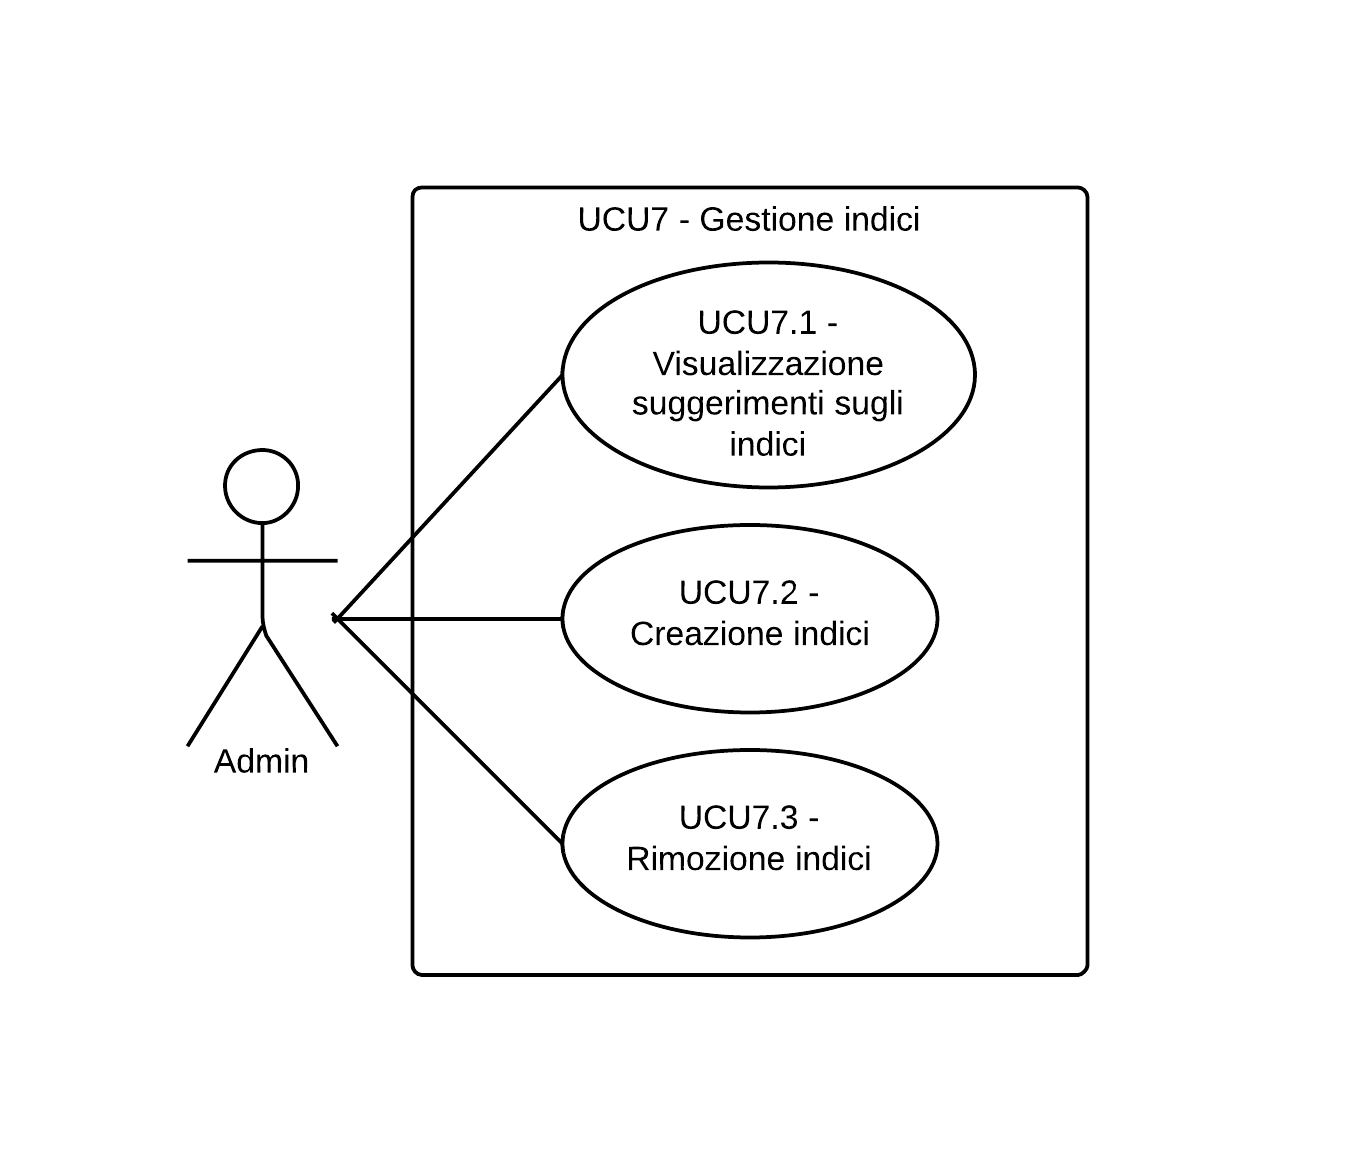
\includegraphics[scale=0.16]{UML/UCU7 - Gestione Indici.png}
      \caption{UCU7 - Gestione Indici} 
    \end{figure}
    \end{center}
    
      %Tabella 
      \begin{center}
      \bgroup
      \def\arraystretch{1.8}     
      \begin{longtable}{  p{3.5cm} | p{8cm} } 
            
      \hline
      \multicolumn{2}{ | c | }{ \cellcolor[gray]{0.9} \textbf{UCU7 - Gestione Indici}} \\ 
      \hline
      
      \textbf{Attori Primari} & Admin \\ 
          \textbf{Scopo e Descrizione} & L'admin può visualizzare i suggerimenti proposti sugli indici e può decidere di aggiungerli. 
Gli indici già presenti possono essere eliminati. \\ 
          
          \textbf{Precondizioni}  & L'applicazione mette a disposizione dell'admin la pagina per gestire gli indici.\\ 
          
          \textbf{Postcondizioni} & L'applicazione ha fornito all'admin le funzionalità di gestione degli indici. \\
          
          \textbf{Flusso Principale} & 1. La pagina di gestione visualizza i suggerimenti per la creazione degli indici (UCU7.1);
2. La pagina di gestione permette all'admin la creazione degli indici suggeriti (UCU7.2);
3. La pagina di gestione permette all'admin l'eliminazione degli indici suggeriti (UCU7.2);
 \\
          
      \end{longtable}
      \egroup
\end{center}

\subsubsection{UCU7.1 - Visualizzazione suggerimenti sugli indici} 
      %Tabella 
      \begin{center}
      \bgroup
      \def\arraystretch{1.8}     
      \begin{longtable}{  p{3.5cm} | p{8cm} } 
            
      \hline
      \multicolumn{2}{ | c | }{ \cellcolor[gray]{0.9} \textbf{UCU7.1 - Visualizzazione suggerimenti sugli indici}} \\ 
      \hline
      
      \textbf{Attori Primari} & Admin \\ 
          \textbf{Scopo e Descrizione} & La pagina di gestione degli indici fornisce all'admin un elenco suggerito di attributi a cui applicare gli indici in base alle query più utilizzate. \\ 
          
          \textbf{Precondizioni}  & L'applicazione ha eseguito una ricerca sulle query più utilizzate. \\ 
          
          \textbf{Postcondizioni} & L'applicazione visualizza correttamente tutti i suggerimenti derivati dalla ricerca. \\
          
          \textbf{Flusso Principale} &  \\
          
      \end{longtable}
      \egroup
\end{center}

\subsubsection{UCU7.2 - Creazione indici} 
      %Tabella 
      \begin{center}
      \bgroup
      \def\arraystretch{1.8}     
      \begin{longtable}{  p{3.5cm} | p{8cm} } 
            
      \hline
      \multicolumn{2}{ | c | }{ \cellcolor[gray]{0.9} \textbf{UCU7.2 - Creazione indici}} \\ 
      \hline
      
      \textbf{Attori Primari} & Admin \\ 
          \textbf{Scopo e Descrizione} & L'Admin seleziona gli indici suggeriti e li crea. \\ 
          
          \textbf{Precondizioni}  & L'applicazione visualizza correttamente la lista degli indici suggeriti\\ 
          
          \textbf{Postcondizioni} & L'applicazione ha creato gli indici selezionati dall'Admin. \\
          
          \textbf{Flusso Principale} &  \\
          
      \end{longtable}
      \egroup
\end{center}

\subsubsection{UCU7.3 - Rimozione indici} 
      %Tabella 
      \begin{center}
      \bgroup
      \def\arraystretch{1.8}     
      \begin{longtable}{  p{3.5cm} | p{8cm} } 
            
      \hline
      \multicolumn{2}{ | c | }{ \cellcolor[gray]{0.9} \textbf{UCU7.3 - Rimozione indici}} \\ 
      \hline
      
      \textbf{Attori Primari} & Admin \\ 
          \textbf{Scopo e Descrizione} & L'Admin seleziona gli indici visualizzati dall'applicazione e li rimuove. \\ 
          
          \textbf{Precondizioni}  & L'applicazione visualizza correttamente la lista degli indici.\\ 
          
          \textbf{Postcondizioni} & L'applicazione ha eliminato gli indici selezionati dall'Admin. \\
          
          \textbf{Flusso Principale} &  \\
          
      \end{longtable}
      \egroup
\end{center}

\subsubsection{UCU8 - Visualizzazione Dashboard} 
      %Tabella 
      \begin{center}
      \bgroup
      \def\arraystretch{1.8}     
      \begin{longtable}{  p{3.5cm} | p{8cm} } 
            
      \hline
      \multicolumn{2}{ | c | }{ \cellcolor[gray]{0.9} \textbf{UCU8 - Visualizzazione Dashboard}} \\ 
      \hline
      
      \textbf{Attori Primari} & Utente autenticato, Admin \\ 
          \textbf{Scopo e Descrizione} & L'utente autenticato può visualizzare la pagina di dashboard. \\ 
          
          \textbf{Precondizioni}  & L'applicazione predispone della pagina di dashboard.\\ 
          
          \textbf{Postcondizioni} & L'applicazione visualizza all'utente la pagina di dashboard. \\
          
          \textbf{Flusso Principale} &  \\
          
      \end{longtable}
      \egroup
\end{center}

\subsubsection{UCU9 - Visualizzazione Collection Index} 
    \begin{center}
    \begin{figure}[H]
      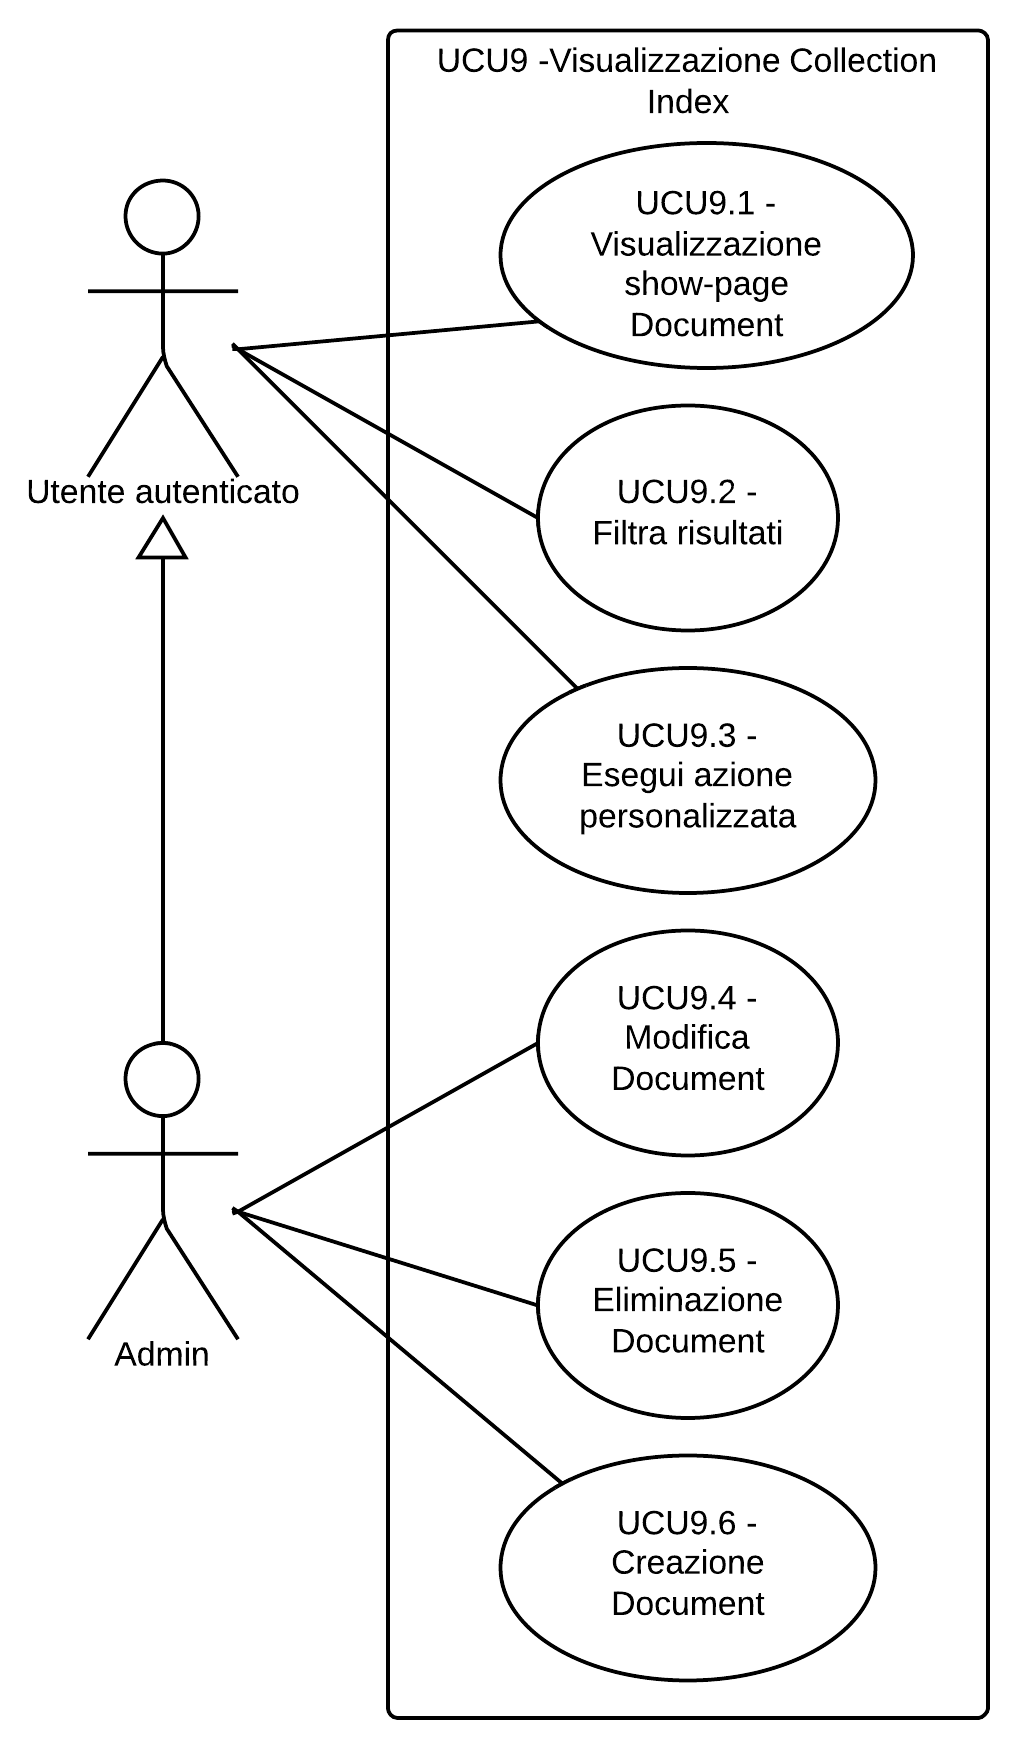
\includegraphics[scale=0.16]{UML/UCU9 - Visualizzazione Collection Index.png}
      \caption{UCU9 - Visualizzazione Collection Index} 
    \end{figure}
    \end{center}
    
      %Tabella 
      \begin{center}
      \bgroup
      \def\arraystretch{1.8}     
      \begin{longtable}{  p{3.5cm} | p{8cm} } 
            
      \hline
      \multicolumn{2}{ | c | }{ \cellcolor[gray]{0.9} \textbf{UCU9 - Visualizzazione Collection Index}} \\ 
      \hline
      
      \textbf{Attori Primari} & Utente autenticato, Admin \\ 
          \textbf{Scopo e Descrizione} & L'utente autenticato , selezionata una collection, ne visualizza in forma tabellare tutti i documenti che contiene.
Di questa collection può filtrarne i risultati visualizzabili, può eseguire tramite bottoni predisposti nella pagina azioni personalizzati e per ogni Document, selezionarlo e visualizzarne la show-page corrispondente.
L'admin ha i permessi per modificare un documento o eliminare un documento. \\ 
          
          \textbf{Precondizioni}  & L'applicazione ha ricevuto la richiesta da parte dell'utente di visualizzazione della collection.\\ 
          
          \textbf{Postcondizioni} & L'applicazione ha visualizzato la collection-index selezionata dall'utente. \\
          
          \textbf{Flusso Principale} &  \\
           \textbf{Scenari Alternativi} & 1. L'utente autenticato può visualizzare la show page relativa ad un Document (UCU9.1);
2. L'utente autenticato può filtrare la collection (UCU9.2);
3. L'utente autenticato può eseguire un'azione personalizzata se è presente (UCU9.3);
4. L'admin può modificare un Document (UCU9.4);
4. L'admin può eliminare un Document (UCU9.5). \\
      \end{longtable}
      \egroup
\end{center}

\subsubsection{UCU9.1 - Visualizzazione show-page Document} 
    \begin{center}
    \begin{figure}[H]
      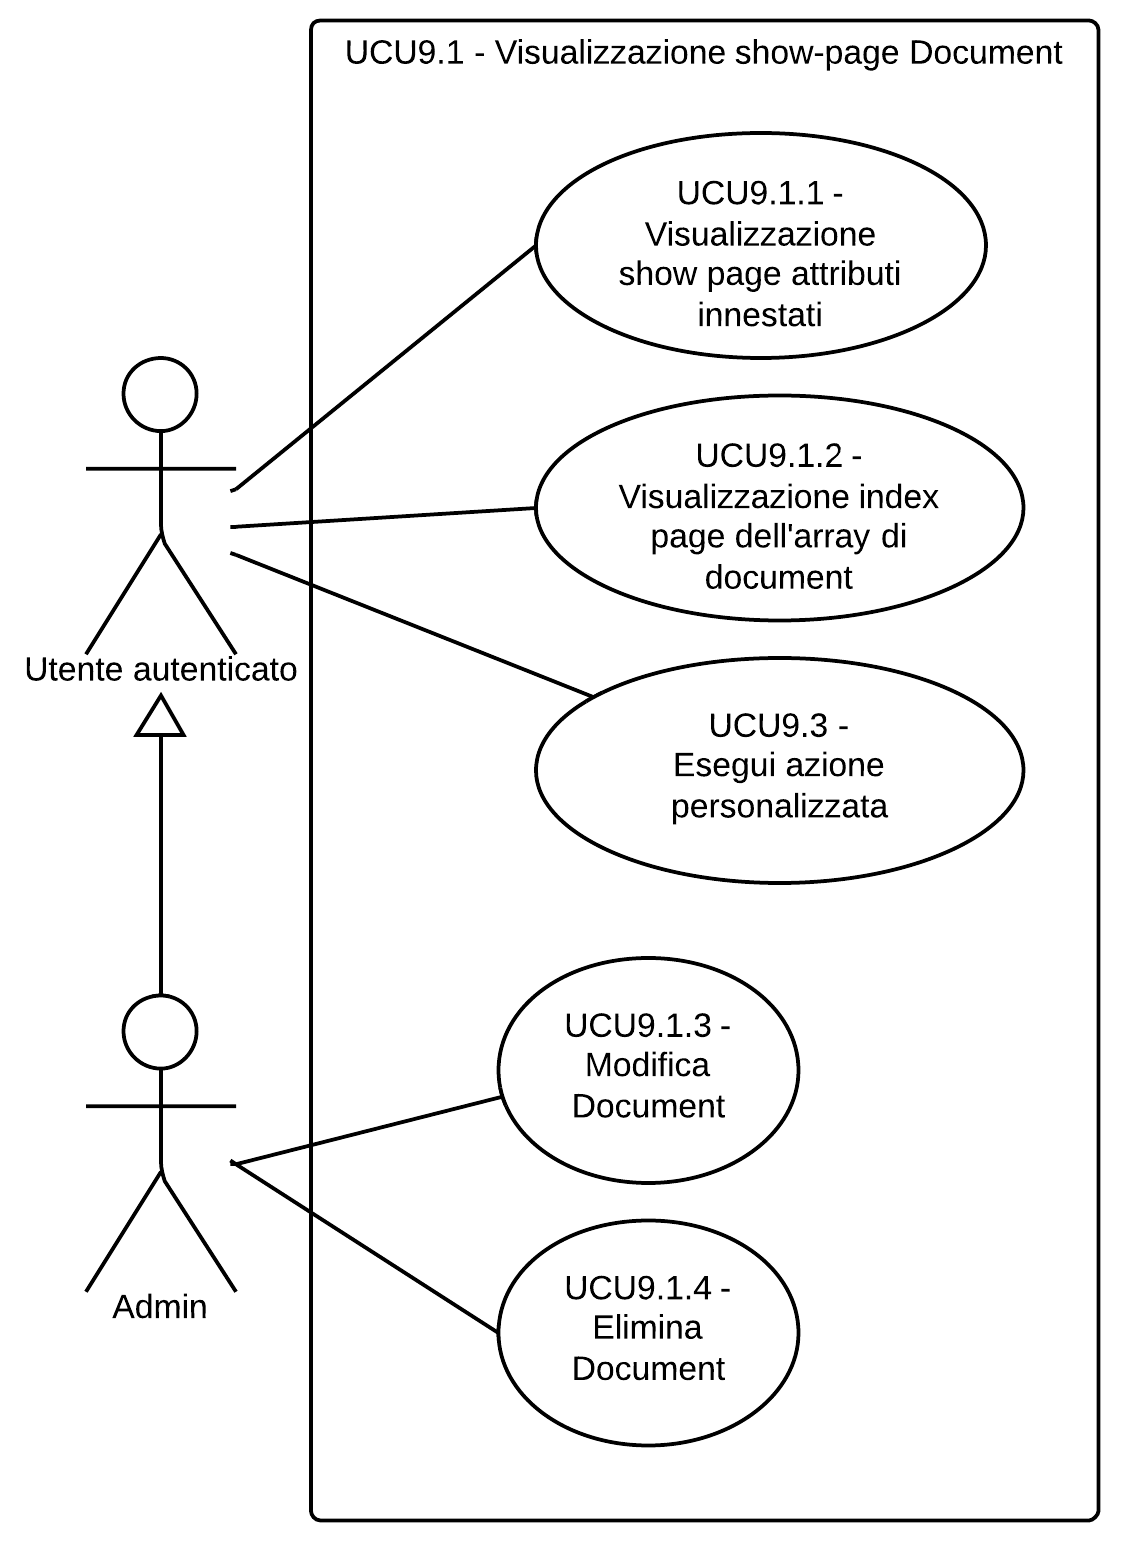
\includegraphics[scale=0.16]{UML/UCU9.1 - Visualizzazione show-page Document.png}
      \caption{UCU9.1 - Visualizzazione show-page Document} 
    \end{figure}
    \end{center}
    
      %Tabella 
      \begin{center}
      \bgroup
      \def\arraystretch{1.8}     
      \begin{longtable}{  p{3.5cm} | p{8cm} } 
            
      \hline
      \multicolumn{2}{ | c | }{ \cellcolor[gray]{0.9} \textbf{UCU9.1 - Visualizzazione show-page Document}} \\ 
      \hline
      
      \textbf{Attori Primari} & Utente autenticato, Admin \\ 
          \textbf{Scopo e Descrizione} & L'utente visualizza la pagina show-page corrispondente ad un Document selezionato visualizzandone gli attributi in forma tabellare.
In questa pagina può aprire la show page o l'index page dell'array di Document degli attributi innestati se presenti, eseguire un'operazione personalizzata se ne sono disponibili.
L'admin può eliminare il Document a cui la show page corrisponde o modificarlo. \\ 
          
          \textbf{Precondizioni}  & L'applicazione ha ottenuto l'informazione necessaria per poter visualizzare la show-page correlata al Document selezionato dall'utente.\\ 
          
          \textbf{Postcondizioni} & L'applicazione mostra all'utente la show-page corrispondente ed è pronta ad eseguire azioni. \\
          
          \textbf{Flusso Principale} & 1. L'utente autenticato può aprire la show page degli attributi innestati. (UCU9.1.1);
2. L'utente autenticato può aprire l'index page dell'array di Document (UCU9.1.2);
3. L'utente autenticato può eseguire se presente un'operazione personalizzata (UCU9.3);
4. L'admin può modificare il Document (UCU9.1.3);
5. L'admin può eliminare il Document (UCU9.1.4). \\
          
      \end{longtable}
      \egroup
\end{center}

\subsubsection{UCU9.1.1 -  Visualizzazione show page attributi innestati} 
      %Tabella 
      \begin{center}
      \bgroup
      \def\arraystretch{1.8}     
      \begin{longtable}{  p{3.5cm} | p{8cm} } 
            
      \hline
      \multicolumn{2}{ | c | }{ \cellcolor[gray]{0.9} \textbf{UCU9.1.1 -  Visualizzazione show page attributi innestati}} \\ 
      \hline
      
      \textbf{Attori Primari} & Utente autenticato, Admin \\ 
          \textbf{Scopo e Descrizione} & L'utente può visualizzare gli attributi degli attributi innestati se presenti del Document. \\ 
          
          \textbf{Precondizioni}  & L'applicazione riceve l'informazione necessaria per visualizzare l'attributo innestato selezionato dall'utente.\\ 
          
          \textbf{Postcondizioni} & L'applicazione visualizza gli attributi dell'attributo innestato. \\
          
          \textbf{Flusso Principale} &  \\
          
      \end{longtable}
      \egroup
\end{center}

\subsubsection{UCU9.1.2 - Visualizzazione index page dell'array di Document} 
      %Tabella 
      \begin{center}
      \bgroup
      \def\arraystretch{1.8}     
      \begin{longtable}{  p{3.5cm} | p{8cm} } 
            
      \hline
      \multicolumn{2}{ | c | }{ \cellcolor[gray]{0.9} \textbf{UCU9.1.2 - Visualizzazione index page dell'array di Document}} \\ 
      \hline
      
      \textbf{Attori Primari} & Utente autenticato, Admin \\ 
          \textbf{Scopo e Descrizione} & L'utente può visualizzare l'index page dell'array di Document. \\ 
          
          \textbf{Precondizioni}  & L'applicazione ha ricevuto la richiesta di visualizzazione dell'index page dell'array di Document dell'attributo selezionato dall'utente.\\ 
          
          \textbf{Postcondizioni} & L'applicazione mostra l'index page dell'array di Document. \\
          
          \textbf{Flusso Principale} &  \\
          
      \end{longtable}
      \egroup
\end{center}

\subsubsection{UCU9.1.3 - Modifica Document} 
      %Tabella 
      \begin{center}
      \bgroup
      \def\arraystretch{1.8}     
      \begin{longtable}{  p{3.5cm} | p{8cm} } 
            
      \hline
      \multicolumn{2}{ | c | }{ \cellcolor[gray]{0.9} \textbf{UCU9.1.3 - Modifica Document}} \\ 
      \hline
      
      \textbf{Attori Primari} & Admin \\ 
          \textbf{Scopo e Descrizione} & L'Admin può modificare gli attributi del Document corrispondente alla page-show visualizzata. \\ 
          
          \textbf{Precondizioni}  & L'applicazione visualizza gli attributi del documento permettendo di modificarli.\\ 
          
          \textbf{Postcondizioni} & L'applicazione ha salvato le modifiche effettuate dall'Admin al Document. \\
          
          \textbf{Flusso Principale} &  \\
           \textbf{Scenari Alternativi} & 1. L'admin annulla le modifiche al Document. \\
      \end{longtable}
      \egroup
\end{center}

\subsubsection{UCU9.1.4 - Elimina Document} 
      %Tabella 
      \begin{center}
      \bgroup
      \def\arraystretch{1.8}     
      \begin{longtable}{  p{3.5cm} | p{8cm} } 
            
      \hline
      \multicolumn{2}{ | c | }{ \cellcolor[gray]{0.9} \textbf{UCU9.1.4 - Elimina Document}} \\ 
      \hline
      
      \textbf{Attori Primari} & Admin \\ 
          \textbf{Scopo e Descrizione} & L'admin può eliminare il Document selezionato nella show-page visualizzata. \\ 
          
          \textbf{Precondizioni}  & L'applicazione permette l'eliminazione del Document.\\ 
          
          \textbf{Postcondizioni} & L'applicazione ha eliminato il Document dalla collection. \\
          
          \textbf{Flusso Principale} &  \\
          
      \end{longtable}
      \egroup
\end{center}

\subsubsection{UCU9.2 - Filtra risultati} 
      %Tabella 
      \begin{center}
      \bgroup
      \def\arraystretch{1.8}     
      \begin{longtable}{  p{3.5cm} | p{8cm} } 
            
      \hline
      \multicolumn{2}{ | c | }{ \cellcolor[gray]{0.9} \textbf{UCU9.2 - Filtra risultati}} \\ 
      \hline
      
      \textbf{Attori Primari} & Utente autenticato, Admin \\ 
          \textbf{Scopo e Descrizione} & L'utente può filtrare i documenti mostrati dalla collection-index. \\ 
          
          \textbf{Precondizioni}  & L'applicazione, nella pagina visualizzata, mette a disposizione filtri.\\ 
          
          \textbf{Postcondizioni} & L'applicazione ha filtrato i documenti visualizzati secondo i filtri richiesti dall'utente. \\
          
          \textbf{Flusso Principale} &  \\
          
      \end{longtable}
      \egroup
\end{center}

\subsubsection{UCU9.3 - Esegui azione personalizzata} 
      %Tabella 
      \begin{center}
      \bgroup
      \def\arraystretch{1.8}     
      \begin{longtable}{  p{3.5cm} | p{8cm} } 
            
      \hline
      \multicolumn{2}{ | c | }{ \cellcolor[gray]{0.9} \textbf{UCU9.3 - Esegui azione personalizzata}} \\ 
      \hline
      
      \textbf{Attori Primari} & Utente autenticato, Admin \\ 
          \textbf{Scopo e Descrizione} & L'utente può eseguire azioni personalizzate tramite uso di bottoni se predisposti nella pagina visualizzata. \\ 
          
          \textbf{Precondizioni}  & L'applicazione  nella pagina visualizzata ha bottoni predisposti per l'esecuzione di azioni personalizzate.\\ 
          
          \textbf{Postcondizioni} & L'applicazione a seconda dell'azione eseguita dall'utente ha svolto le sue funzioni. \\
          
          \textbf{Flusso Principale} &  \\
          
      \end{longtable}
      \egroup
\end{center}

\subsubsection{UCU9.4 - Modifica Document} 
      %Tabella 
      \begin{center}
      \bgroup
      \def\arraystretch{1.8}     
      \begin{longtable}{  p{3.5cm} | p{8cm} } 
            
      \hline
      \multicolumn{2}{ | c | }{ \cellcolor[gray]{0.9} \textbf{UCU9.4 - Modifica Document}} \\ 
      \hline
      
      \textbf{Attori Primari} & Admin \\ 
          \textbf{Scopo e Descrizione} & L'admin può selezionare un Document per andarlo a modificare. \\ 
          
          \textbf{Precondizioni}  & L'applicazione mostra in forma tabellare tutti i Document della collection predisponendo la possibilità per ognuno di modifica.\\ 
          
          \textbf{Postcondizioni} & L'applicazione ha salvato le modifiche apportate dall'utente al Document. \\
          
          \textbf{Flusso Principale} &  \\
           \textbf{Scenari Alternativi} & 1. L'admin non ha modificato il Document. \\
      \end{longtable}
      \egroup
\end{center}

\subsubsection{UCU9.5 - Elimina Document} 
      %Tabella 
      \begin{center}
      \bgroup
      \def\arraystretch{1.8}     
      \begin{longtable}{  p{3.5cm} | p{8cm} } 
            
      \hline
      \multicolumn{2}{ | c | }{ \cellcolor[gray]{0.9} \textbf{UCU9.5 - Elimina Document}} \\ 
      \hline
      
      \textbf{Attori Primari} & Admin \\ 
          \textbf{Scopo e Descrizione} & L'admin può eliminare un Document direttamente dalla pagina collection index visualizzata. \\ 
          
          \textbf{Precondizioni}  & L'applicazione ha predisposto per ogni Document visualizzato nella collection, la possibilità di eliminarlo.\\ 
          
          \textbf{Postcondizioni} & L'applicazione ha eliminato il Document selezionato dalla collection. \\
          
          \textbf{Flusso Principale} &  \\
          
      \end{longtable}
      \egroup
\end{center}

\subsubsection{UCU9.6 - Creazione Document} 
      %Tabella 
      \begin{center}
      \bgroup
      \def\arraystretch{1.8}     
      \begin{longtable}{  p{3.5cm} | p{8cm} } 
            
      \hline
      \multicolumn{2}{ | c | }{ \cellcolor[gray]{0.9} \textbf{UCU9.6 - Creazione Document}} \\ 
      \hline
      
      \textbf{Attori Primari} & Admin \\ 
          \textbf{Scopo e Descrizione} & L'admin può creare un nuovo Document. \\ 
          
          \textbf{Precondizioni}  & L'Applicazione è pronta a gestire le richieste dell'utente admin e permette la creazione di nuovi Document.\\ 
          
          \textbf{Postcondizioni} & L'Applicazione Maap ha creato il nuovo Document. \\
          
          \textbf{Flusso Principale} &  \\
          
      \end{longtable}
      \egroup
\end{center}

\subsubsection{UCU10 - Modifica profilo} 
    \begin{center}
    \begin{figure}[H]
      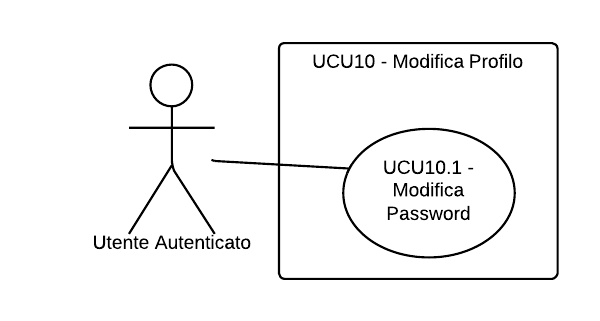
\includegraphics[scale=0.16]{UML/UCU10 - Modifica profilo.png}
      \caption{UCU10 - Modifica profilo} 
    \end{figure}
    \end{center}
    
      %Tabella 
      \begin{center}
      \bgroup
      \def\arraystretch{1.8}     
      \begin{longtable}{  p{3.5cm} | p{8cm} } 
            
      \hline
      \multicolumn{2}{ | c | }{ \cellcolor[gray]{0.9} \textbf{UCU10 - Modifica profilo}} \\ 
      \hline
      
      \textbf{Attori Primari} & Utente autenticato \\ 
          \textbf{Scopo e Descrizione} & L'utente autenticato ha a disposizione una pagina in cui poter modificare il proprio profilo, modificando email e/o password. \\ 
          
          \textbf{Precondizioni}  & L'utente si trova all'interno della pagina di modifica del proprio profilo.\\ 
          
          \textbf{Postcondizioni} & L'utente ha modificato il proprio profilo e il database è stato aggiornato. \\
          
          \textbf{Flusso Principale} & 1. L'utente autenticato modifica la propria email (UCU10.1);
2. L'utente autenticato modifica la propria password (UCU10.2); \\
          
      \end{longtable}
      \egroup
\end{center}

\subsubsection{UCU10.1 - Modifica email} 
      %Tabella 
      \begin{center}
      \bgroup
      \def\arraystretch{1.8}     
      \begin{longtable}{  p{3.5cm} | p{8cm} } 
            
      \hline
      \multicolumn{2}{ | c | }{ \cellcolor[gray]{0.9} \textbf{UCU10.1 - Modifica email}} \\ 
      \hline
      
      \textbf{Attori Primari} & Utente autenticato \\ 
          \textbf{Scopo e Descrizione} & L'utente autenticato inserisce la nuova email in un apposito campo di testo. \\ 
          
          \textbf{Precondizioni}  & L'utente autenticato si trova all'interno della pagina di modifica del proprio profilo.\\ 
          
          \textbf{Postcondizioni} & L'utente ha inserito la nuova email all'interno dell'apposito campo. \\
          
          \textbf{Flusso Principale} &  \\
          
      \end{longtable}
      \egroup
\end{center}

\subsubsection{UCU10.2 - Modifica password} 
      %Tabella 
      \begin{center}
      \bgroup
      \def\arraystretch{1.8}     
      \begin{longtable}{  p{3.5cm} | p{8cm} } 
            
      \hline
      \multicolumn{2}{ | c | }{ \cellcolor[gray]{0.9} \textbf{UCU10.2 - Modifica password}} \\ 
      \hline
      
      \textbf{Attori Primari} & Utente autenticato \\ 
          \textbf{Scopo e Descrizione} & L'utente autenticato inserisce la nuova password in un apposito campo di testo. \\ 
          
          \textbf{Precondizioni}  & L'utente autenticato si trova all'interno della pagina di modifica del proprio profilo.\\ 
          
          \textbf{Postcondizioni} & L'utente ha inserito la nuova password all'interno dell'apposito campo. \\
          
          \textbf{Flusso Principale} &  \\
          
      \end{longtable}
      \egroup
\end{center}

\subsubsection{UCU11 - Gestione utenti} 
    \begin{center}
    \begin{figure}[H]
      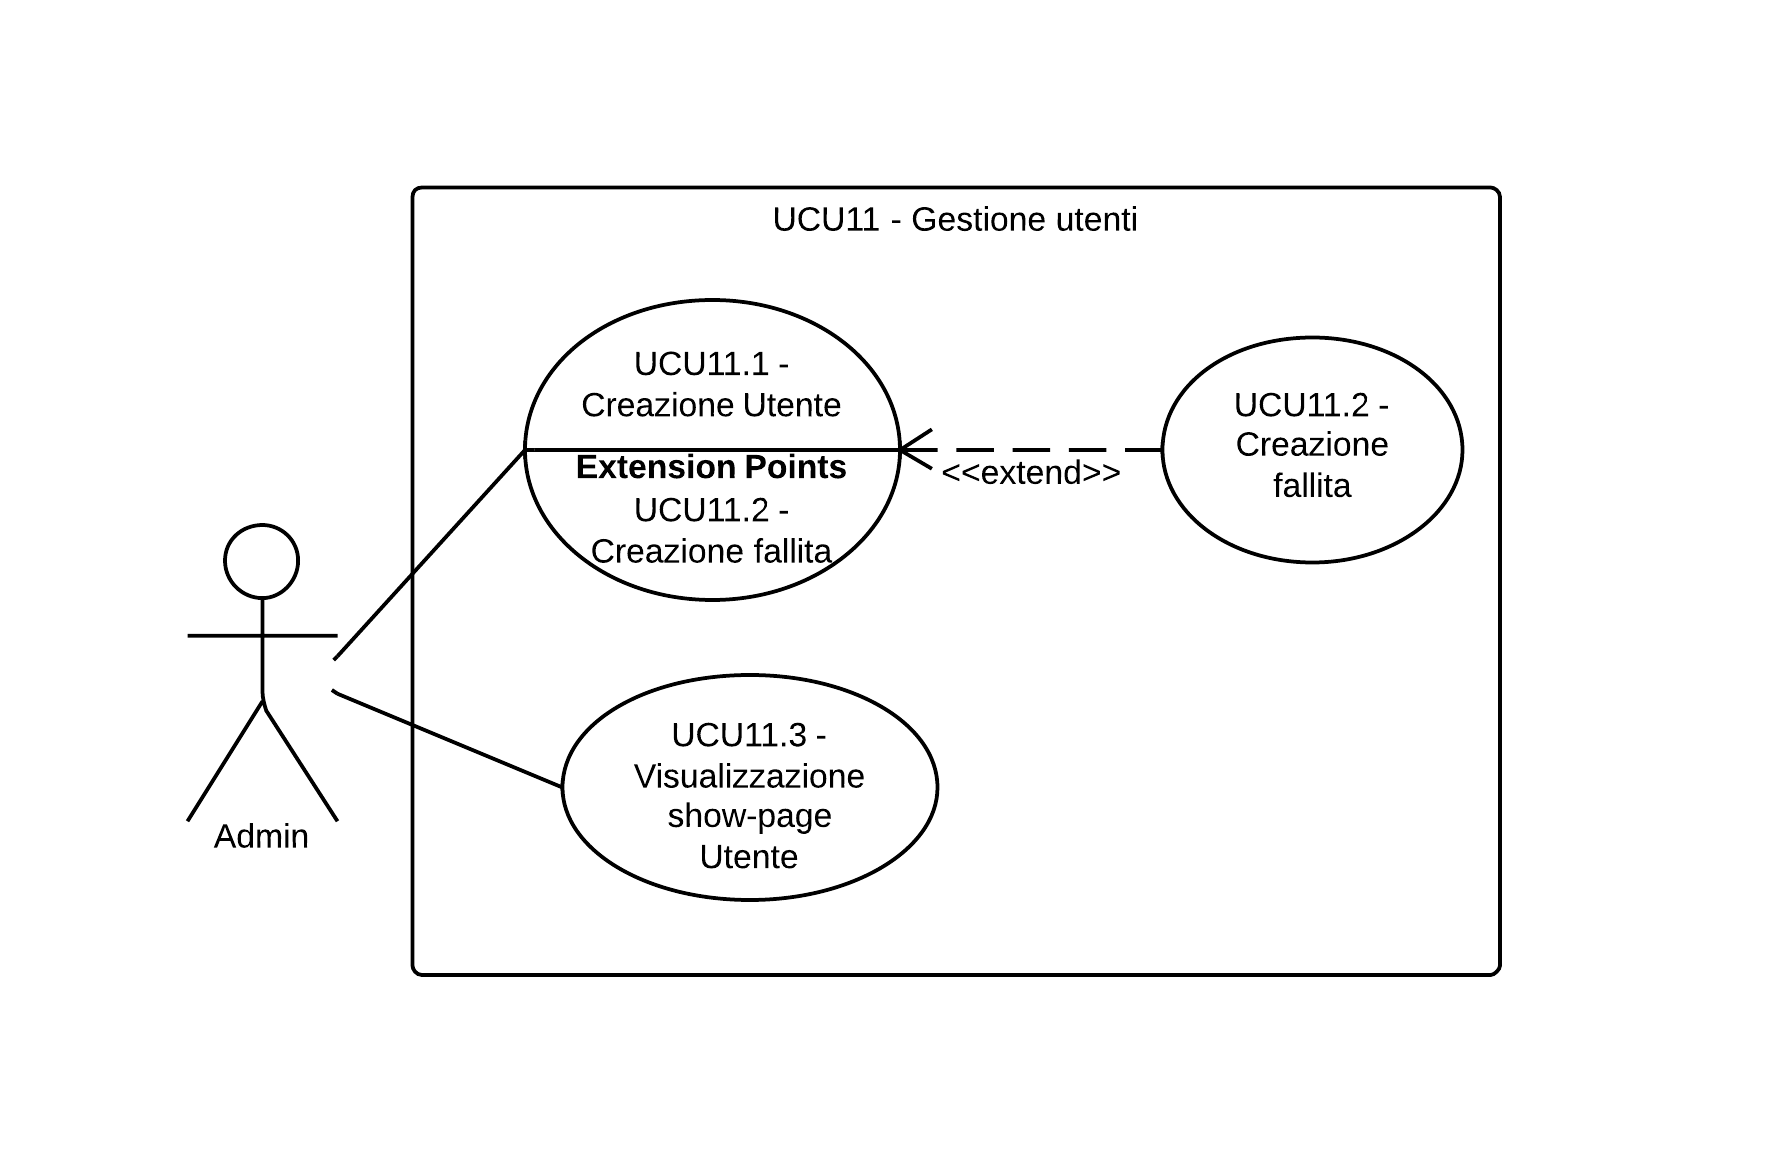
\includegraphics[scale=0.16]{UML/UCU11 - Gestione utenti.png}
      \caption{UCU11 - Gestione utenti} 
    \end{figure}
    \end{center}
    
      %Tabella 
      \begin{center}
      \bgroup
      \def\arraystretch{1.8}     
      \begin{longtable}{  p{3.5cm} | p{8cm} } 
            
      \hline
      \multicolumn{2}{ | c | }{ \cellcolor[gray]{0.9} \textbf{UCU11 - Gestione utenti}} \\ 
      \hline
      
      \textbf{Attori Primari} & Admin \\ 
          \textbf{Scopo e Descrizione} & L'admin entra nella sua pagina di amministrazione dalla quale visualizza una Collection-index di tutti gli utenti registrati al sistema. \\ 
          
          \textbf{Precondizioni}  & Il sistema mostra all'admin la sua pagina di amministrazione\\ 
          
          \textbf{Postcondizioni} & Il sistema mette a disposizione dell'admin tutte le funzionalità di controllo previste. \\
          
          \textbf{Flusso Principale} & 1. L'admin può creare un nuovo utente (UCU11.1)
2. L'admin può visualizzare la Collection-show di un utente (UCU11.3) \\
           \textbf{Esclusioni} & 1.1 - Fallisce l'inserimento di un nuovo utente (UCU11.2). \\
      \end{longtable}
      \egroup
\end{center}

\subsubsection{UCU11.1 - Creazione utente} 
    \begin{center}
    \begin{figure}[H]
      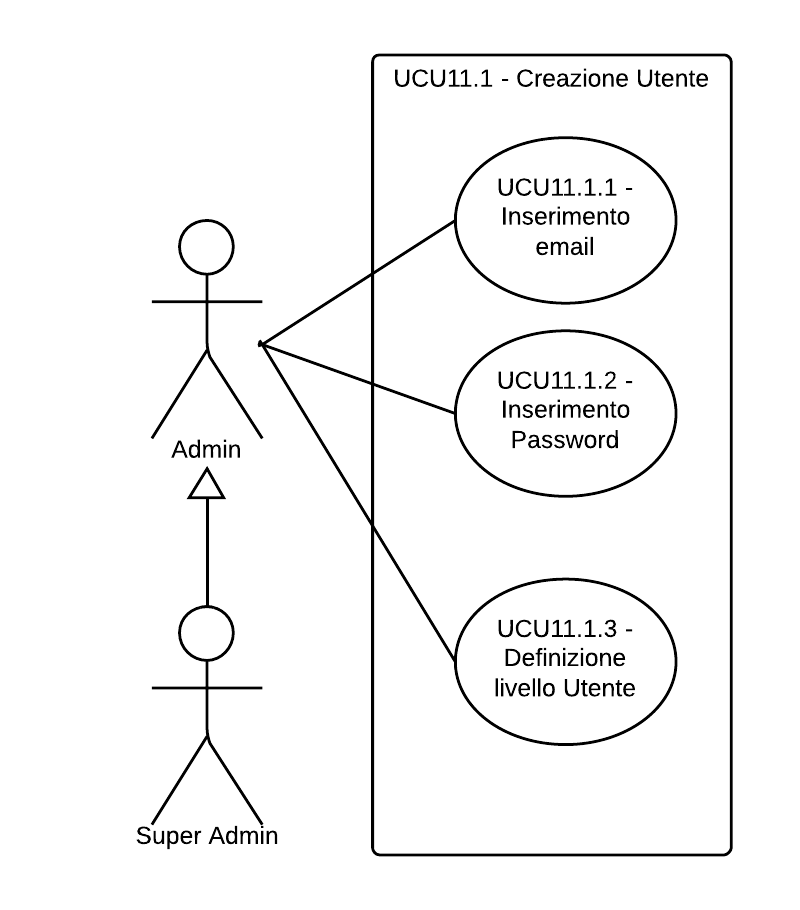
\includegraphics[scale=0.16]{UML/UCU11.1 - Creazione utente.png}
      \caption{UCU11.1 - Creazione utente} 
    \end{figure}
    \end{center}
    
      %Tabella 
      \begin{center}
      \bgroup
      \def\arraystretch{1.8}     
      \begin{longtable}{  p{3.5cm} | p{8cm} } 
            
      \hline
      \multicolumn{2}{ | c | }{ \cellcolor[gray]{0.9} \textbf{UCU11.1 - Creazione utente}} \\ 
      \hline
      
      \textbf{Attori Primari} & Admin \\ 
          \textbf{Scopo e Descrizione} & L'admin entra in un'apposita pagina di creazione utente, dalla quale inserisce i dati e crea un nuovo utente nel database. \\ 
          
          \textbf{Precondizioni}  & Il sistema ha reindirizzato l'admin nella pagina di creazione di un nuovo utente.\\ 
          
          \textbf{Postcondizioni} & Il sistema ha creato un nuovo utente nel database con i dati immessi dall'admin. \\
          
          \textbf{Flusso Principale} & 1. L'admin inserisce l'indirizzo email del nuovo utente (UCU11.1.1);
2. L'admin inserisce la password del nuovo utente (UCU11.1.2); 
3. L'admin definisce il livello del nuovo utente (UCU11.1.3). \\
           \textbf{Scenari Alternativi} & 1. L'admin lascia la pagina senza aver salvato le modifiche;
2. I dati inseriti dall'admin non sono corretti e fallisce la registrazione. \\
      \end{longtable}
      \egroup
\end{center}

\subsubsection{UCU11.1.1 - Inserimento email} 
      %Tabella 
      \begin{center}
      \bgroup
      \def\arraystretch{1.8}     
      \begin{longtable}{  p{3.5cm} | p{8cm} } 
            
      \hline
      \multicolumn{2}{ | c | }{ \cellcolor[gray]{0.9} \textbf{UCU11.1.1 - Inserimento email}} \\ 
      \hline
      
      \textbf{Attori Primari} & Admin \\ 
          \textbf{Scopo e Descrizione} & L'admin può inserire in un campo di testo l'indirizzo email dell'utente da creare. \\ 
          
          \textbf{Precondizioni}  & Il sistema mette a disposizione dell'admin un campo di testo dove inserire la password del nuovo utente.\\ 
          
          \textbf{Postcondizioni} & Il campo di testo è stato compilato correttamente. \\
          
          \textbf{Flusso Principale} &  \\
          
      \end{longtable}
      \egroup
\end{center}

\subsubsection{UCU11.1.2 - Inserimento password} 
      %Tabella 
      \begin{center}
      \bgroup
      \def\arraystretch{1.8}     
      \begin{longtable}{  p{3.5cm} | p{8cm} } 
            
      \hline
      \multicolumn{2}{ | c | }{ \cellcolor[gray]{0.9} \textbf{UCU11.1.2 - Inserimento password}} \\ 
      \hline
      
      \textbf{Attori Primari} & Admin \\ 
          \textbf{Scopo e Descrizione} & L'admin può inserire in un campo di testo la password dell'utente da creare. \\ 
          
          \textbf{Precondizioni}  & L'admin è nella pagina di creazione di un nuovo utente.\\ 
          
          \textbf{Postcondizioni} & L'admin ha inserito l'indirizzo email dell'utente da creare. \\
          
          \textbf{Flusso Principale} &  \\
          
      \end{longtable}
      \egroup
\end{center}

\subsubsection{UCU11.1.3 - Definizione livello utente} 
      %Tabella 
      \begin{center}
      \bgroup
      \def\arraystretch{1.8}     
      \begin{longtable}{  p{3.5cm} | p{8cm} } 
            
      \hline
      \multicolumn{2}{ | c | }{ \cellcolor[gray]{0.9} \textbf{UCU11.1.3 - Definizione livello utente}} \\ 
      \hline
      
      \textbf{Attori Primari} & Admin \\ 
          \textbf{Scopo e Descrizione} & L'admin può selezionare il livello del nuovo utente, che potrà essere utente normale o admin. \\ 
          
          \textbf{Precondizioni}  & Il sistema mette a disposizione dell'admin un campo selezionabile dove poter definire il livello del nuovo utente.\\ 
          
          \textbf{Postcondizioni} & Il campo selezionabile è stato selezionato correttamente. \\
          
          \textbf{Flusso Principale} &  \\
          
      \end{longtable}
      \egroup
\end{center}

\subsubsection{UCU11.2 - Creazione fallita} 
      %Tabella 
      \begin{center}
      \bgroup
      \def\arraystretch{1.8}     
      \begin{longtable}{  p{3.5cm} | p{8cm} } 
            
      \hline
      \multicolumn{2}{ | c | }{ \cellcolor[gray]{0.9} \textbf{UCU11.2 - Creazione fallita}} \\ 
      \hline
      
      \textbf{Attori Primari} & Admin \\ 
          \textbf{Scopo e Descrizione} & L'admin ha inserito delle credenziali errate e la creazione di un nuovo utente è fallita. \\ 
          
          \textbf{Precondizioni}  & Il sistema ha rilevato degli errori nell'inserimento di un nuovo utente.\\ 
          
          \textbf{Postcondizioni} & Il sistema visualizza un messaggio d'errore. \\
          
          \textbf{Flusso Principale} &  \\
          
      \end{longtable}
      \egroup
\end{center}

\subsubsection{UCU11.3 - Visualizzazione show-page Utente} 
    \begin{center}
    \begin{figure}[H]
      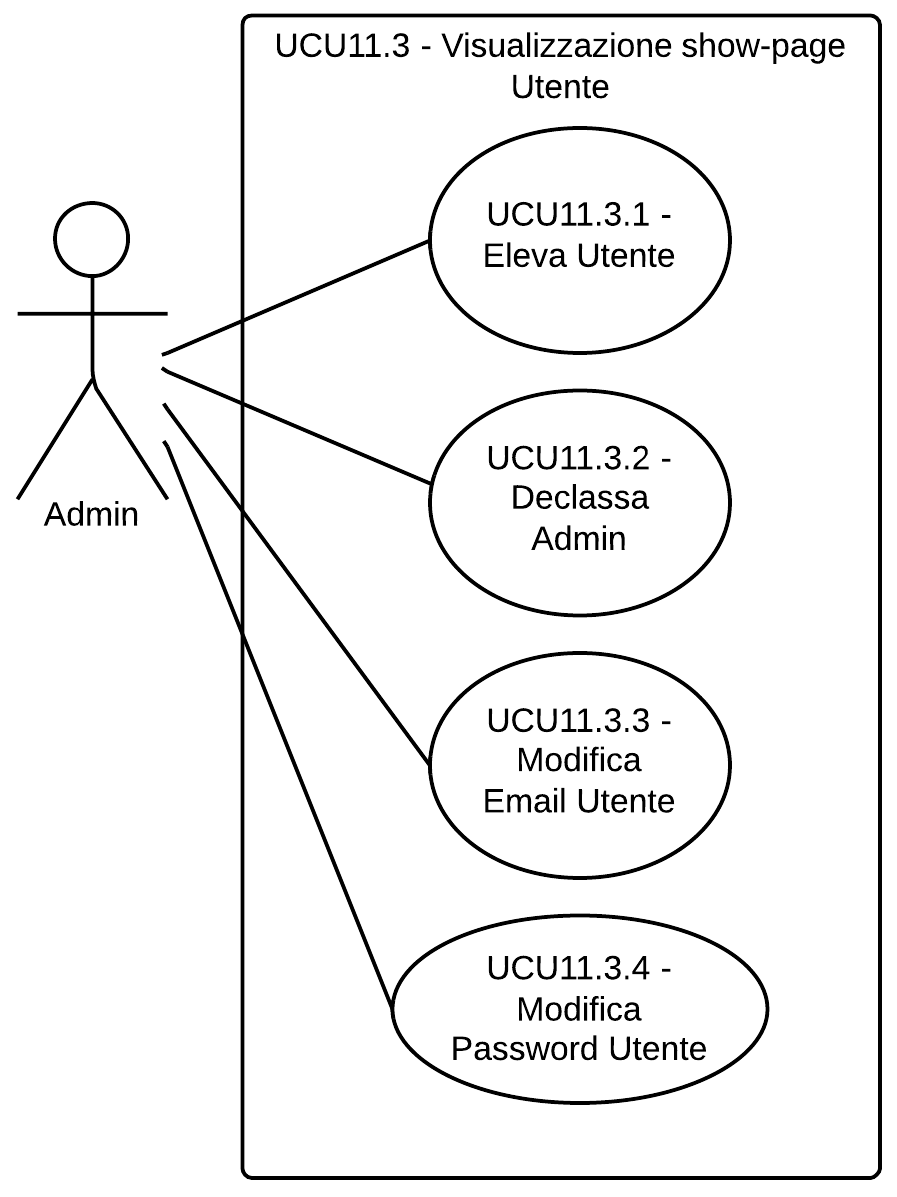
\includegraphics[scale=0.16]{UML/UCU11.3 - Visualizzazione show-page Utente.png}
      \caption{UCU11.3 - Visualizzazione show-page Utente} 
    \end{figure}
    \end{center}
    
      %Tabella 
      \begin{center}
      \bgroup
      \def\arraystretch{1.8}     
      \begin{longtable}{  p{3.5cm} | p{8cm} } 
            
      \hline
      \multicolumn{2}{ | c | }{ \cellcolor[gray]{0.9} \textbf{UCU11.3 - Visualizzazione show-page Utente}} \\ 
      \hline
      
      \textbf{Attori Primari} & Admin \\ 
          \textbf{Scopo e Descrizione} & L'admin visualizza la tabella degli utenti registrati e può aprire la relativa show-page di uno di essi tramite link. \\ 
          
          \textbf{Precondizioni}  & L'applicazione mette a disposizione dell'admin la visualizzazione della show-index dell'utente.\\ 
          
          \textbf{Postcondizioni} & L'applicazione MaaP ha reindirizzato l'admin nella Collection-show dell'utente selezionato. \\
          
          \textbf{Flusso Principale} & 1. L'admin può elevare un utente normale a livello di admin (UCU11.3.1);
2. L'admin può declassare un admin a livello di utente normale (UCU11.3.2);
3. L'admin può modificare l'email dell'utente selezionato (UCU11.3.3);
4. L'admin può modificare la password dell'utente selezionato (UCU11.3.4); \\
          
      \end{longtable}
      \egroup
\end{center}

\subsubsection{UCU11.3.1 - Eleva utente} 
      %Tabella 
      \begin{center}
      \bgroup
      \def\arraystretch{1.8}     
      \begin{longtable}{  p{3.5cm} | p{8cm} } 
            
      \hline
      \multicolumn{2}{ | c | }{ \cellcolor[gray]{0.9} \textbf{UCU11.3.1 - Eleva utente}} \\ 
      \hline
      
      \textbf{Attori Primari} & Admin \\ 
          \textbf{Scopo e Descrizione} & L'admin eleva l'utente selezionato a livello di admin. \\ 
          
          \textbf{Precondizioni}  & L'applicazione MaaP mette a disposizione dell'admin la pagina di modifica dell'utente selezionato.\\ 
          
          \textbf{Postcondizioni} & L'applicazione MaaP ha elevato l'utente selezionato dall'admin a livello di admin. \\
          
          \textbf{Flusso Principale} &  \\
          
      \end{longtable}
      \egroup
\end{center}

\subsubsection{UCU11.3.2 - Declassa admin} 
      %Tabella 
      \begin{center}
      \bgroup
      \def\arraystretch{1.8}     
      \begin{longtable}{  p{3.5cm} | p{8cm} } 
            
      \hline
      \multicolumn{2}{ | c | }{ \cellcolor[gray]{0.9} \textbf{UCU11.3.2 - Declassa admin}} \\ 
      \hline
      
      \textbf{Attori Primari} & Admin \\ 
          \textbf{Scopo e Descrizione} & L'admin declassa l'admin selezionato al livello di utente normale. \\ 
          
          \textbf{Precondizioni}  & L'applicazione MaaP mette a disposizione dell'admin la pagina di modifica dell'utente selezionato.\\ 
          
          \textbf{Postcondizioni} & L'applicazione MaaP ha declassato l'utente selezionato dall'admin a livello di utente normale. \\
          
          \textbf{Flusso Principale} &  \\
          
      \end{longtable}
      \egroup
\end{center}

\subsubsection{UCU11.3.3 - Modifica email utente} 
      %Tabella 
      \begin{center}
      \bgroup
      \def\arraystretch{1.8}     
      \begin{longtable}{  p{3.5cm} | p{8cm} } 
            
      \hline
      \multicolumn{2}{ | c | }{ \cellcolor[gray]{0.9} \textbf{UCU11.3.3 - Modifica email utente}} \\ 
      \hline
      
      \textbf{Attori Primari} & Admin \\ 
          \textbf{Scopo e Descrizione} & L'admin modifica l'email dell'utente selezionato. \\ 
          
          \textbf{Precondizioni}  & L'applicazione MaaP mette a disposizione dell'admin la pagina di modifica dell'utente selezionato.\\ 
          
          \textbf{Postcondizioni} & L'applicazione MaaP ha modificato l'indirizzo email dell'utente selezionato dall'admin. \\
          
          \textbf{Flusso Principale} &  \\
          
      \end{longtable}
      \egroup
\end{center}

\subsubsection{UCU11.3.4 - Modifica Password Utente} 
      %Tabella 
      \begin{center}
      \bgroup
      \def\arraystretch{1.8}     
      \begin{longtable}{  p{3.5cm} | p{8cm} } 
            
      \hline
      \multicolumn{2}{ | c | }{ \cellcolor[gray]{0.9} \textbf{UCU11.3.4 - Modifica Password Utente}} \\ 
      \hline
      
      \textbf{Attori Primari} & Admin \\ 
          \textbf{Scopo e Descrizione} & L'admin può modificare la password dell'utente corrispondente alla show-page visualizzata. \\ 
          
          \textbf{Precondizioni}  & L'applicazione MaaP mette a disposizione dell'admin la pagina di modifica dell'utente selezionato.\\ 
          
          \textbf{Postcondizioni} & L'applicazione ha modificato la password dell'utente relativo alla show-page corrispondente. \\
          
          \textbf{Flusso Principale} &  \\
          
      \end{longtable}
      \egroup
\end{center}
\subsection{Ambito Sviluppatore}
\subsubsection{UCS - Operazioni ad alto livello} 
    \begin{center}
    \begin{figure}[H]
      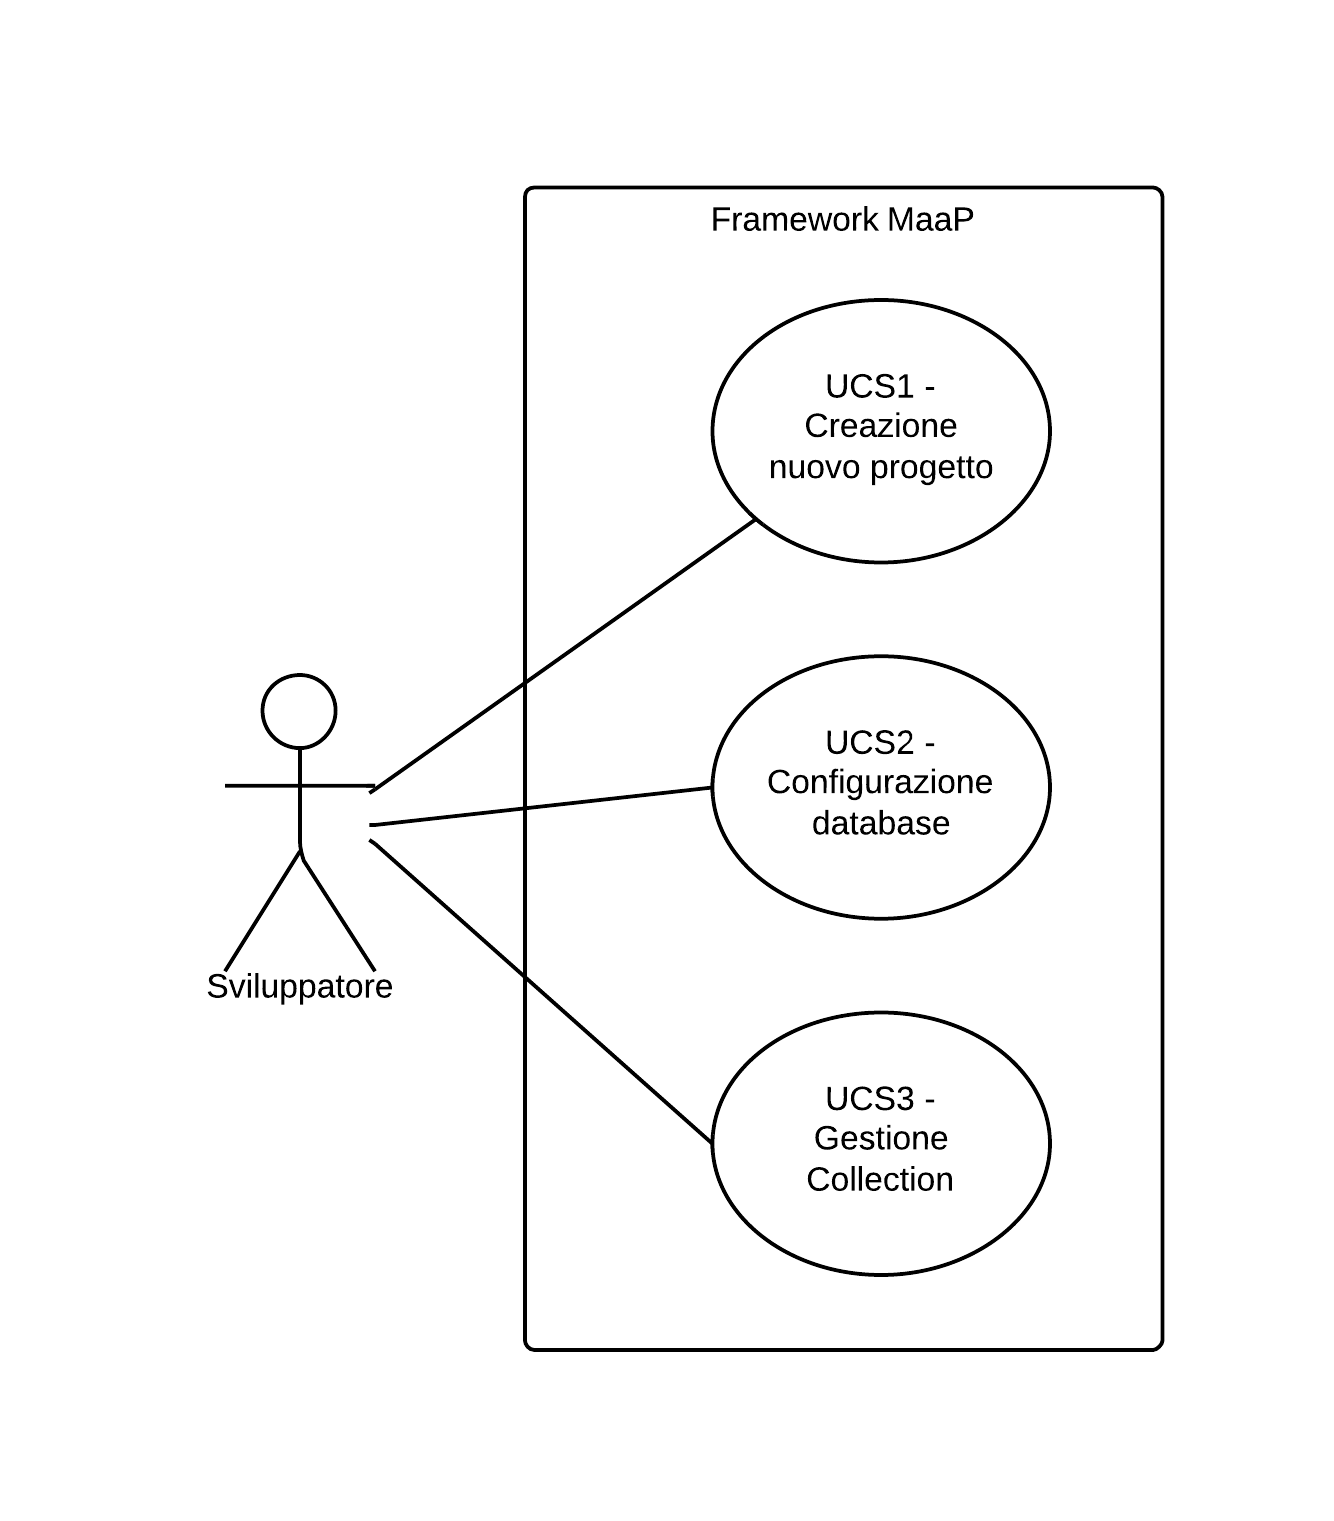
\includegraphics[scale=0.16]{UML/UCS - Operazioni ad alto livello.png}
      \caption{UCS - Operazioni ad alto livello} 
    \end{figure}
    \end{center}
    
      %Tabella 
      \begin{center}
      \bgroup
      \def\arraystretch{1.8}     
      \begin{longtable}{  p{3.5cm} | p{8cm} } 
            
      \hline
      \multicolumn{2}{ | c | }{ \cellcolor[gray]{0.9} \textbf{UCS - Operazioni ad alto livello}} \\ 
      \hline
      
      \textbf{Attori Primari} & Sviluppatore \\ 
          \textbf{Scopo e Descrizione} & Lo sviluppatore avendo installato lo stack tecnologico richiesto per il funzionamento del Framework Maap può creare un nuovo progetto, dopo averlo creato potrà configurare i database e gestire le collection che desidera. \\ 
          
          \textbf{Precondizioni}  & Il Framework Maap è funzionante e pronto ad eseguire le azioni dello sviluppatore.\\ 
          
          \textbf{Postcondizioni} & Il Framework ha ottenuto le informazioni sulle azioni che l’utente desidera eseguire. \\
          
          \textbf{Flusso Principale} & 1. Lo Sviluppatore crea un nuovo progetto (UCS1);
2. Lo sviluppatore dopo aver creato il nuovo progetto può configurare i database (UCS2);
3. Lo sviluppatore con il nuovo progetto creato può gestire le collection che desidera generare (UCS3). \\
          
      \end{longtable}
      \egroup
\end{center}

\subsubsection{UCS1 - Creazione nuovo progetto} 
      %Tabella 
      \begin{center}
      \bgroup
      \def\arraystretch{1.8}     
      \begin{longtable}{  p{3.5cm} | p{8cm} } 
            
      \hline
      \multicolumn{2}{ | c | }{ \cellcolor[gray]{0.9} \textbf{UCS1 - Creazione nuovo progetto}} \\ 
      \hline
      
      \textbf{Attori Primari} & Sviluppatore \\ 
          \textbf{Scopo e Descrizione} & Lo sviluppatore crea un nuovo progetto.
Alla creazione del nuovo progetto ne viene creato lo scheletro che si compone di:
- La creazione delle directory delle pagine web.
- La creazione del file di configurazione.
- L'inclusione delle librerie di sistema.
- La generazione del sistema di autenticazione che include la creazione del database delle credenziali e la generazione dell'utente admin di default. \\ 
          
          \textbf{Precondizioni}  & Il Framework è pronto a creare un nuovo progetto.\\ 
          
          \textbf{Postcondizioni} & Il Framework Maap ha creato un nuovo progetto completo di tutti i file necessari. \\
          
          \textbf{Flusso Principale} &  \\
          
      \end{longtable}
      \egroup
\end{center}

\subsubsection{UCS2 - Configurazione database} 
      %Tabella 
      \begin{center}
      \bgroup
      \def\arraystretch{1.8}     
      \begin{longtable}{  p{3.5cm} | p{8cm} } 
            
      \hline
      \multicolumn{2}{ | c | }{ \cellcolor[gray]{0.9} \textbf{UCS2 - Configurazione database}} \\ 
      \hline
      
      \textbf{Attori Primari} & Sviluppatore \\ 
          \textbf{Scopo e Descrizione} & Lo sviluppatore può configurare i due database che compongono il sistema Maap, ovvero il database delle credenziali utenti e il database contenente le collection. \\ 
          
          \textbf{Precondizioni}  & Framework è funzionante, il progetto è stato creato e lo sviluppatore desidera configurare i database.\\ 
          
          \textbf{Postcondizioni} & Il Framework ha ottenuto le informazioni necessarie ed ha configurato il database delle credenziali e il database delle collection. \\
          
          \textbf{Flusso Principale} &  \\
          
      \end{longtable}
      \egroup
\end{center}

\subsubsection{UCS2.1 - Configurazione database credenziali} 
      %Tabella 
      \begin{center}
      \bgroup
      \def\arraystretch{1.8}     
      \begin{longtable}{  p{3.5cm} | p{8cm} } 
            
      \hline
      \multicolumn{2}{ | c | }{ \cellcolor[gray]{0.9} \textbf{UCS2.1 - Configurazione database credenziali}} \\ 
      \hline
      
      \textbf{Attori Primari} & Sviluppatore \\ 
          \textbf{Scopo e Descrizione} & Lo sviluppatore può configurare il database che conterrà le credenziali degli utenti i quali utilizzeranno l'applicazione generata dal Framework. \\ 
          
          \textbf{Precondizioni}  & Il Framework permette la configurazione del database credenziali.\\ 
          
          \textbf{Postcondizioni} & Il Framework Maap ha configurato il database delle credenziali secondo le informazioni acquisite dallo sviluppatore. \\
          
          \textbf{Flusso Principale} &  \\
          
      \end{longtable}
      \egroup
\end{center}

\subsubsection{UCS2.2 - Configurazione database Collection} 
      %Tabella 
      \begin{center}
      \bgroup
      \def\arraystretch{1.8}     
      \begin{longtable}{  p{3.5cm} | p{8cm} } 
            
      \hline
      \multicolumn{2}{ | c | }{ \cellcolor[gray]{0.9} \textbf{UCS2.2 - Configurazione database Collection}} \\ 
      \hline
      
      \textbf{Attori Primari} &  \\ 
          \textbf{Scopo e Descrizione} & Lo sviluppatore può configurare il database che conterrà le collection che l'applicazione generata dal Framework utilizzerà. \\ 
          
          \textbf{Precondizioni}  & Il Framework permette la configurazione del database collection.\\ 
          
          \textbf{Postcondizioni} & Il Framework Maap ha configurato il database delle collection secondo le informazioni acquisite dallo sviluppatore. \\
          
          \textbf{Flusso Principale} &  \\
          
      \end{longtable}
      \egroup
\end{center}

\subsubsection{UCS2.3 - Selezione namespace} 
      %Tabella 
      \begin{center}
      \bgroup
      \def\arraystretch{1.8}     
      \begin{longtable}{  p{3.5cm} | p{8cm} } 
            
      \hline
      \multicolumn{2}{ | c | }{ \cellcolor[gray]{0.9} \textbf{UCS2.3 - Selezione namespace}} \\ 
      \hline
      
      \textbf{Attori Primari} & Sviluppatore \\ 
          \textbf{Scopo e Descrizione} & Se la funzione di namespace è abilitata lo sviluppatore può selezionare un namespace per il database da configurare. \\ 
          
          \textbf{Precondizioni}  & Il framework MaaP mette a disposizione dello sviluppatore un file di configurazione del database.\\ 
          
          \textbf{Postcondizioni} & Il framework MaaP ha selezionato correttamente il namespace per il database selezionato. \\
          
          \textbf{Flusso Principale} &  \\
          
      \end{longtable}
      \egroup
\end{center}

\subsubsection{UCS3 - Gestione Collection} 
    \begin{center}
    \begin{figure}[H]
      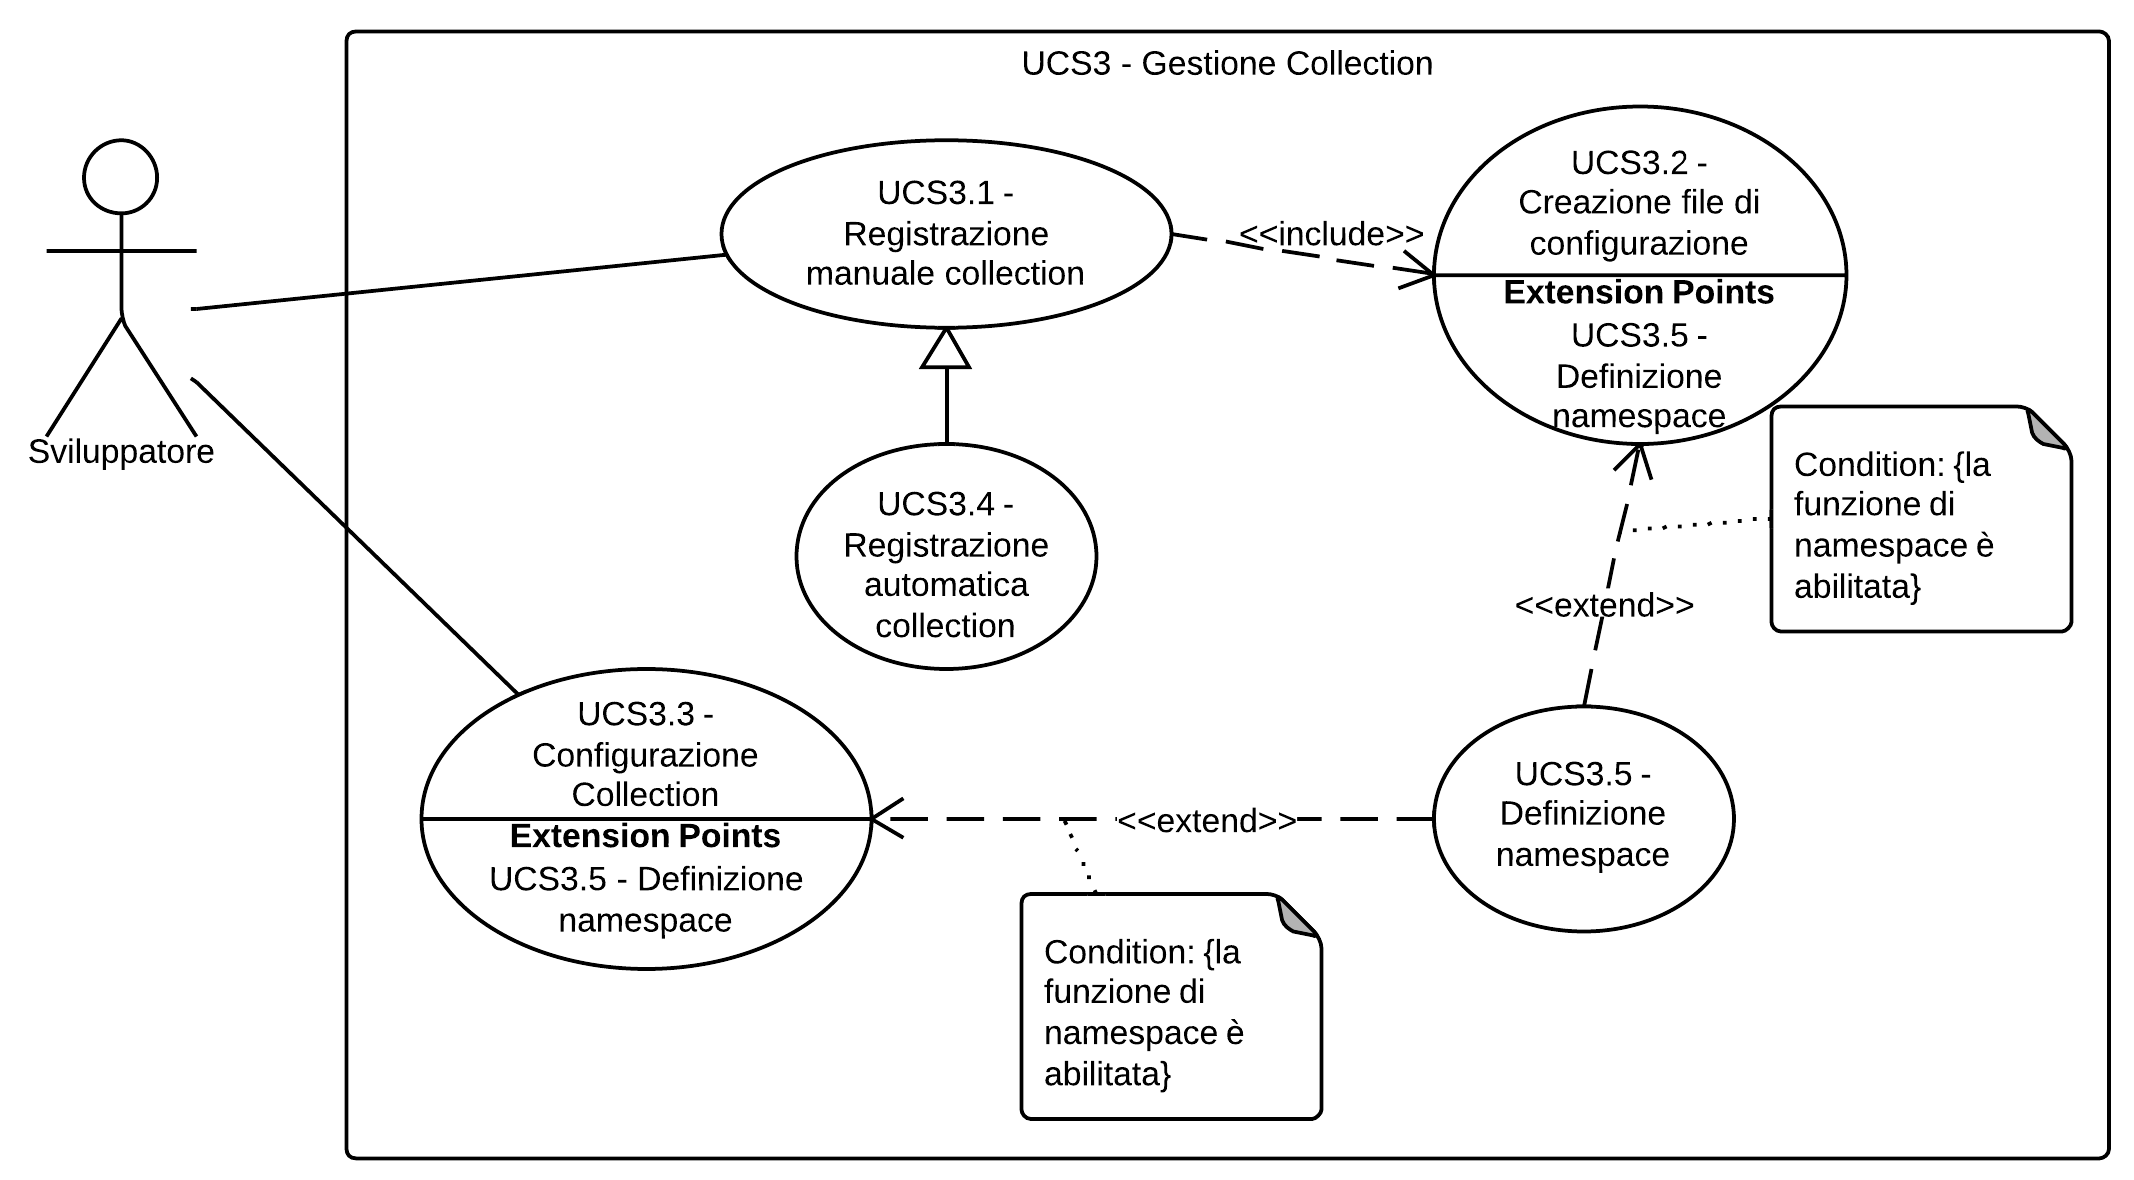
\includegraphics[scale=0.16]{UML/UCS3 - Gestione Collection.png}
      \caption{UCS3 - Gestione Collection} 
    \end{figure}
    \end{center}
    
      %Tabella 
      \begin{center}
      \bgroup
      \def\arraystretch{1.8}     
      \begin{longtable}{  p{3.5cm} | p{8cm} } 
            
      \hline
      \multicolumn{2}{ | c | }{ \cellcolor[gray]{0.9} \textbf{UCS3 - Gestione Collection}} \\ 
      \hline
      
      \textbf{Attori Primari} & Sviluppatore \\ 
          \textbf{Scopo e Descrizione} & Lo sviluppatore, con il progetto creato, può registrare manualmente una collection o usufruire della registrazione automatica, con relativa creazione del file di configurazione della stessa.
Può poi configurare le collection create. \\ 
          
          \textbf{Precondizioni}  & Il Framework MaaP è pronto, il progetto è stato creato e lo sviluppatore intende gestire collection.\\ 
          
          \textbf{Postcondizioni} & Il Framework ha appreso le informazioni necessarie sulle azioni che lo sviluppatore vuole eseguire. \\
          
          \textbf{Flusso Principale} & 1. Lo sviluppatore può registrare manualmente la collection (UCS3.1);
2. Lo sviluppatore può configurare la collection registrata (UCS3.3). \\
           \textbf{Inclusioni} & Viene creato il file di configurazione (UCS3.2). \\ \textbf{Esclusioni} & 1.1. Lo sviluppatore non esegue la registrazione manuale ma eseguire la registrazione automatica della collection (UCS3.4) \\
      \end{longtable}
      \egroup
\end{center}

\subsubsection{UCS3.1 - Registrazione manuale Collection} 
      %Tabella 
      \begin{center}
      \bgroup
      \def\arraystretch{1.8}     
      \begin{longtable}{  p{3.5cm} | p{8cm} } 
            
      \hline
      \multicolumn{2}{ | c | }{ \cellcolor[gray]{0.9} \textbf{UCS3.1 - Registrazione manuale Collection}} \\ 
      \hline
      
      \textbf{Attori Primari} & Sviluppatore \\ 
          \textbf{Scopo e Descrizione} & Lo sviluppatore registra manualmente una Collection creando tutti i file necessari al suo funzionamento. \\ 
          
          \textbf{Precondizioni}  & Il Framework MaaP è funzionante e lo sviluppatore ha creato un progetto.\\ 
          
          \textbf{Postcondizioni} & Il Framework MaaP ha registrato correttamente la nuova Collection. \\
          
          \textbf{Flusso Principale} &  \\
          
      \end{longtable}
      \egroup
\end{center}

\subsubsection{UCS3.2 - Creazione file di configurazione} 
      %Tabella 
      \begin{center}
      \bgroup
      \def\arraystretch{1.8}     
      \begin{longtable}{  p{3.5cm} | p{8cm} } 
            
      \hline
      \multicolumn{2}{ | c | }{ \cellcolor[gray]{0.9} \textbf{UCS3.2 - Creazione file di configurazione}} \\ 
      \hline
      
      \textbf{Attori Primari} & Sviluppatore \\ 
          \textbf{Scopo e Descrizione} & Nella registrazione di una nuova Collection deve essere creato un file di configurazione per essa. \\ 
          
          \textbf{Precondizioni}  & Il Framework MaaP sta registrando una nuova Collection.\\ 
          
          \textbf{Postcondizioni} & Il Framework MaaP ha creato il file di configurazione per la nuova Collection. \\
          
          \textbf{Flusso Principale} &  \\
          
      \end{longtable}
      \egroup
\end{center}

\subsubsection{UCS3.3 - Configurazione Collection} 
    \begin{center}
    \begin{figure}[H]
      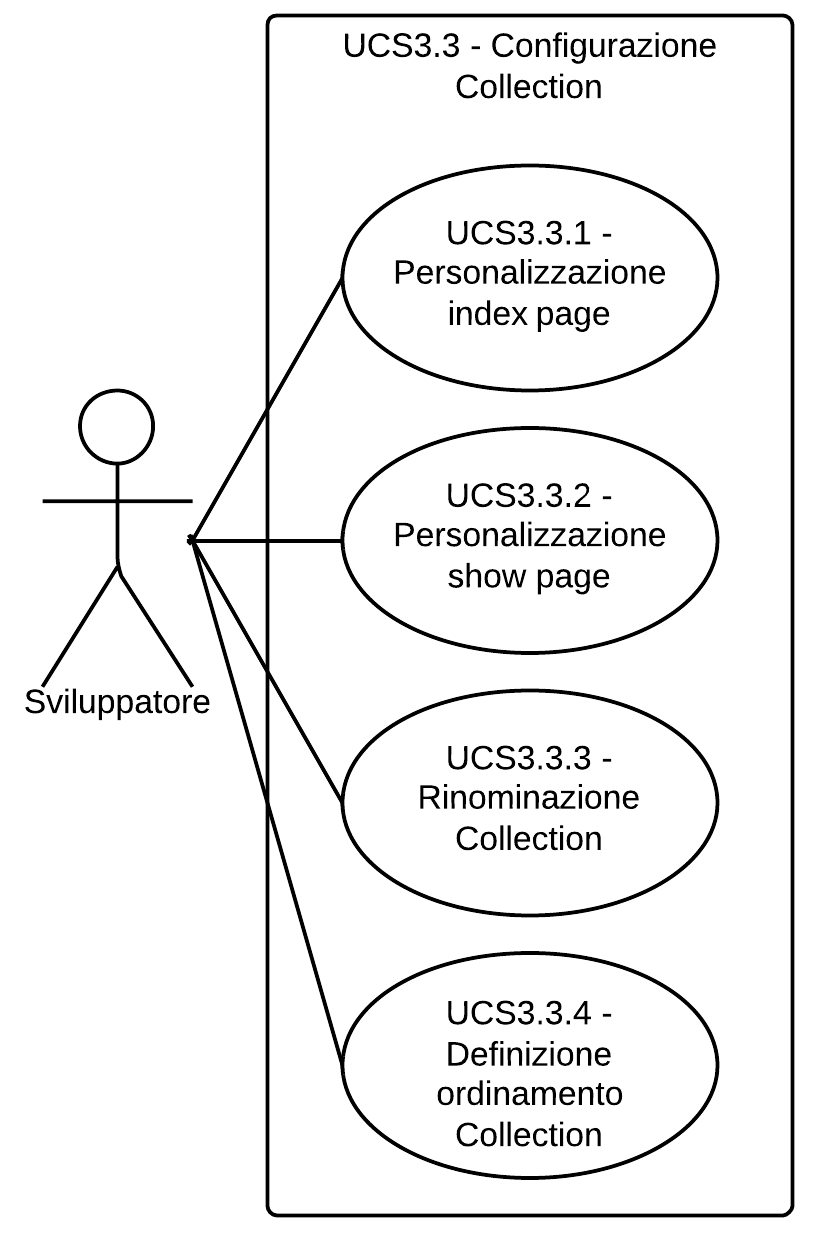
\includegraphics[scale=0.16]{UML/UCS3.3 - Configurazione Collection.png}
      \caption{UCS3.3 - Configurazione Collection} 
    \end{figure}
    \end{center}
    
      %Tabella 
      \begin{center}
      \bgroup
      \def\arraystretch{1.8}     
      \begin{longtable}{  p{3.5cm} | p{8cm} } 
            
      \hline
      \multicolumn{2}{ | c | }{ \cellcolor[gray]{0.9} \textbf{UCS3.3 - Configurazione Collection}} \\ 
      \hline
      
      \textbf{Attori Primari} & Sviluppatore \\ 
          \textbf{Scopo e Descrizione} & Lo sviluppatore modifica il file di configurazione di una Collection creata. \\ 
          
          \textbf{Precondizioni}  & Il Framework MaaP ha registrato correttamente la Collection da configurare.\\ 
          
          \textbf{Postcondizioni} & Il Framework MaaP ha configurato correttamente la Collection modificata dallo sviluppatore. \\
          
          \textbf{Flusso Principale} & 1. Lo sviluppatore personalizza la index page della Collection (UCS3.3.1);
2. Lo sviluppatore personalizza la show page della Collection (UCS3.3.2);
3. Lo sviluppatore rinomina il titolo della Collection che verrà visualizzato nel menu di navigazione (UCS3.3.3);
4. Lo sviluppatore definisce l'ordine di visualizzazione della Collection nel menu di navigazione (UCS3.3.4); \\
          
      \end{longtable}
      \egroup
\end{center}

\subsubsection{UCS3.3.1 - Personalizzazione index page} 
    \begin{center}
    \begin{figure}[H]
      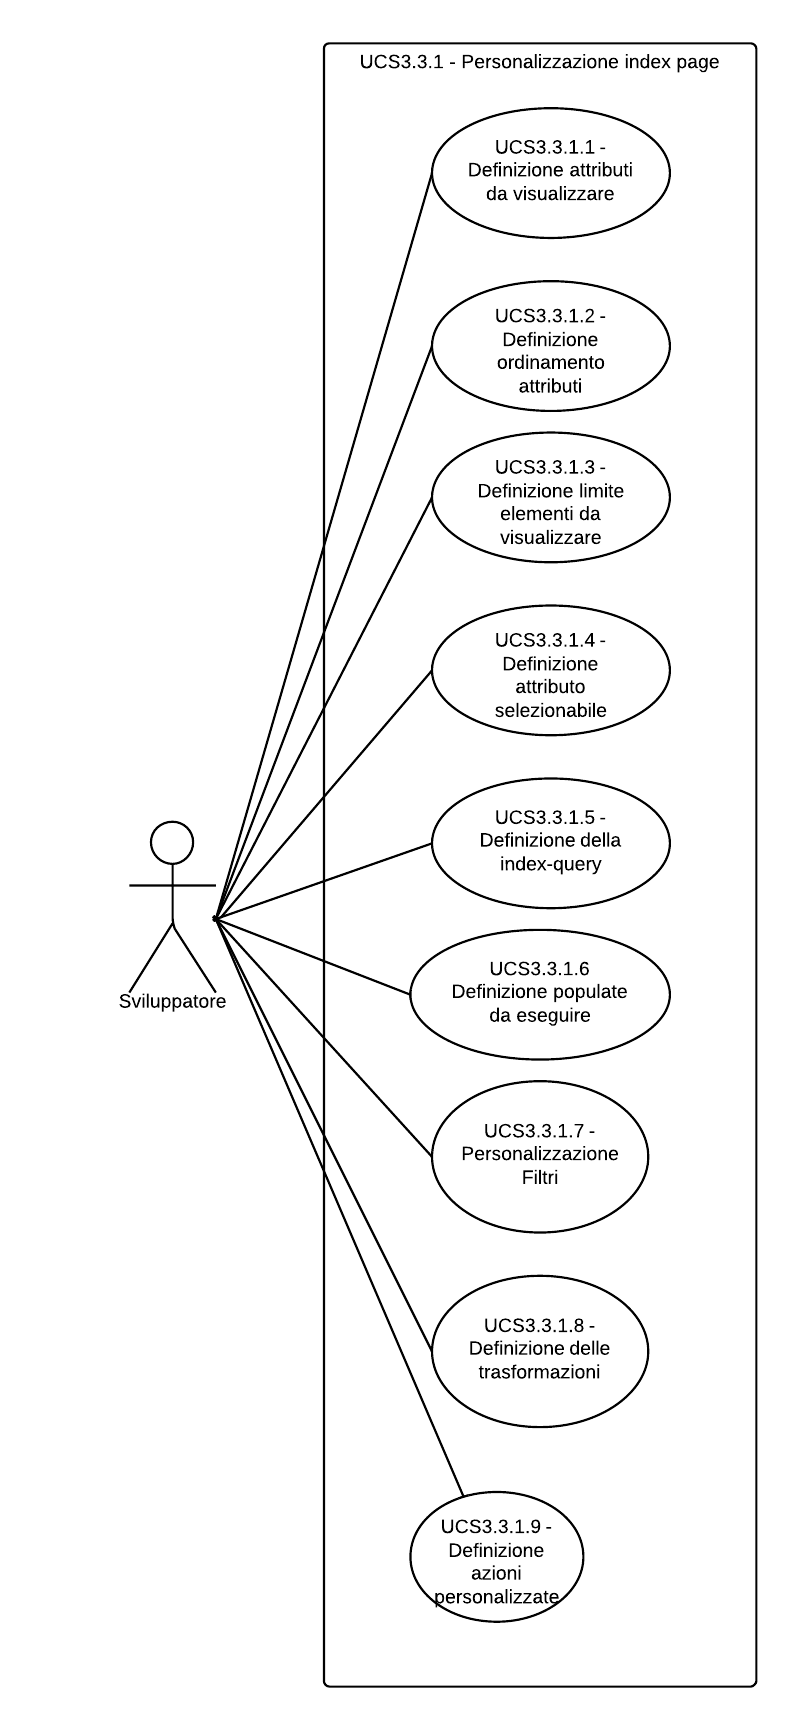
\includegraphics[scale=0.16]{UML/UCS3.3.1 - Personalizzazione index page.png}
      \caption{UCS3.3.1 - Personalizzazione index page} 
    \end{figure}
    \end{center}
    
      %Tabella 
      \begin{center}
      \bgroup
      \def\arraystretch{1.8}     
      \begin{longtable}{  p{3.5cm} | p{8cm} } 
            
      \hline
      \multicolumn{2}{ | c | }{ \cellcolor[gray]{0.9} \textbf{UCS3.3.1 - Personalizzazione index page}} \\ 
      \hline
      
      \textbf{Attori Primari} & Sviluppatore \\ 
          \textbf{Scopo e Descrizione} & Lo sviluppatore personalizza la index page della Collection selezionata. \\ 
          
          \textbf{Precondizioni}  & Il Framework MaaP è funzionante e la Collection da configurare è stata registrata.\\ 
          
          \textbf{Postcondizioni} & Il Framework MaaP ha configurato correttamente la index page della Collection. \\
          
          \textbf{Flusso Principale} & 1. Lo sviluppatore definisce gli attributi da visualizzare (UCS3.3.1.1);
2. Lo sviluppatore definisce l'ordinamento degli attributi (UCS3.3.1.2);
3. Lo sviluppatore definisce il limite degli elementi da visualizzare (UCS3.3.1.3);
4. Lo sviluppatore definisce quale attributo è selezionabile (UCS3.3.1.4);
5. Lo sviluppatore definisce una query che visualizzerà un sottoinsieme di Document dalla Collection (UCS3.3.1.5);
6. Lo sviluppatore definisce come attributo un attributo innestato o un array di attributi (UCS3.3u.1.6);
7. Lo sviluppatore personalizza la tipologia di filtri da visualizzare (UCS3.3.1.7);
8. Lo sviluppatore definisce delle trasformazioni sugli attributi (UCS3.3.1.8);
9. Lo sviluppatore definisce delle azioni personalizzate (UCS3.3.1.9). \\
          
      \end{longtable}
      \egroup
\end{center}

\subsubsection{UCS3.3.1.1 - Definizione attributi da visualizzare} 
      %Tabella 
      \begin{center}
      \bgroup
      \def\arraystretch{1.8}     
      \begin{longtable}{  p{3.5cm} | p{8cm} } 
            
      \hline
      \multicolumn{2}{ | c | }{ \cellcolor[gray]{0.9} \textbf{UCS3.3.1.1 - Definizione attributi da visualizzare}} \\ 
      \hline
      
      \textbf{Attori Primari} & Sviluppatore \\ 
          \textbf{Scopo e Descrizione} & Lo sviluppatore all'interno del file di configurazione della Collection specifica quali attributi visualizzare nella index page. \\ 
          
          \textbf{Precondizioni}  & Il Framework MaaP è funzionante e la Collection è registrata.\\ 
          
          \textbf{Postcondizioni} & Il Framework MaaP ha apportato le modifiche alla configurazione della Collection. \\
          
          \textbf{Flusso Principale} &  \\
          
      \end{longtable}
      \egroup
\end{center}

\subsubsection{UCS3.3.1.2 - Definizione ordinamento attributi} 
      %Tabella 
      \begin{center}
      \bgroup
      \def\arraystretch{1.8}     
      \begin{longtable}{  p{3.5cm} | p{8cm} } 
            
      \hline
      \multicolumn{2}{ | c | }{ \cellcolor[gray]{0.9} \textbf{UCS3.3.1.2 - Definizione ordinamento attributi}} \\ 
      \hline
      
      \textbf{Attori Primari} & Sviluppatore \\ 
          \textbf{Scopo e Descrizione} & Lo sviluppatore all'interno del file di configurazione della Collection definisce un ordinamento di default e specifica quali attributi sono ordinabili o no. \\ 
          
          \textbf{Precondizioni}  & Il Framework MaaP è funzionante e la Collection è registrata.\\ 
          
          \textbf{Postcondizioni} & Il Framework MaaP ha apportato le modifiche alla configurazione della Collection. \\
          
          \textbf{Flusso Principale} &  \\
          
      \end{longtable}
      \egroup
\end{center}

\subsubsection{UCS3.3.1.3 - Definizione limite elementi da visualizzare} 
      %Tabella 
      \begin{center}
      \bgroup
      \def\arraystretch{1.8}     
      \begin{longtable}{  p{3.5cm} | p{8cm} } 
            
      \hline
      \multicolumn{2}{ | c | }{ \cellcolor[gray]{0.9} \textbf{UCS3.3.1.3 - Definizione limite elementi da visualizzare}} \\ 
      \hline
      
      \textbf{Attori Primari} & Sviluppatore \\ 
          \textbf{Scopo e Descrizione} & Lo sviluppatore all'interno del file di configurazione della Collection specifica quanti Document per pagina verranno visualizzati nella index page. \\ 
          
          \textbf{Precondizioni}  & Il Framework MaaP è funzionante e la Collection è registrata.\\ 
          
          \textbf{Postcondizioni} & Il Framework MaaP ha apportato le modifiche alla configurazione della Collection. \\
          
          \textbf{Flusso Principale} &  \\
          
      \end{longtable}
      \egroup
\end{center}

\subsubsection{UCS3.3.1.4 - Definizione attributo selezionabile} 
      %Tabella 
      \begin{center}
      \bgroup
      \def\arraystretch{1.8}     
      \begin{longtable}{  p{3.5cm} | p{8cm} } 
            
      \hline
      \multicolumn{2}{ | c | }{ \cellcolor[gray]{0.9} \textbf{UCS3.3.1.4 - Definizione attributo selezionabile}} \\ 
      \hline
      
      \textbf{Attori Primari} & Sviluppatore \\ 
          \textbf{Scopo e Descrizione} & Lo sviluppatore all'interno del file di configurazione della Collection specifica quale attributo sarà identificato come chiave per poter accedere alla show page del corrispondente Document. \\ 
          
          \textbf{Precondizioni}  & Il Framework MaaP è funzionante e la Collection è registrata.\\ 
          
          \textbf{Postcondizioni} & Il Framework MaaP ha apportato le modifiche alla configurazione della Collection. \\
          
          \textbf{Flusso Principale} &  \\
          
      \end{longtable}
      \egroup
\end{center}

\subsubsection{UCS3.3.1.5 - Definizione della index-query} 
      %Tabella 
      \begin{center}
      \bgroup
      \def\arraystretch{1.8}     
      \begin{longtable}{  p{3.5cm} | p{8cm} } 
            
      \hline
      \multicolumn{2}{ | c | }{ \cellcolor[gray]{0.9} \textbf{UCS3.3.1.5 - Definizione della index-query}} \\ 
      \hline
      
      \textbf{Attori Primari} & Sviluppatore \\ 
          \textbf{Scopo e Descrizione} & Lo sviluppatore all'interno del file di configurazione della Collection definisce delle query che andranno a selezionare un sottoinsieme di Document dalla Collection. \\ 
          
          \textbf{Precondizioni}  & Il Framework MaaP è funzionante e la Collection è registrata.\\ 
          
          \textbf{Postcondizioni} & Il Framework MaaP ha apportato le modifiche alla configurazione della Collection. \\
          
          \textbf{Flusso Principale} &  \\
          
      \end{longtable}
      \egroup
\end{center}

\subsubsection{UCS3.3.1.6 - Definizione populate da eseguire} 
      %Tabella 
      \begin{center}
      \bgroup
      \def\arraystretch{1.8}     
      \begin{longtable}{  p{3.5cm} | p{8cm} } 
            
      \hline
      \multicolumn{2}{ | c | }{ \cellcolor[gray]{0.9} \textbf{UCS3.3.1.6 - Definizione populate da eseguire}} \\ 
      \hline
      
      \textbf{Attori Primari} & Sviluppatore \\ 
          \textbf{Scopo e Descrizione} & Lo sviluppatore all'interno del file di configurazione della Collection specifica attributi che contengono attributi innestati o un array di Document tramite la funzione populate. \\ 
          
          \textbf{Precondizioni}  & Il Framework MaaP è funzionante e la Collection è registrata.\\ 
          
          \textbf{Postcondizioni} & Il Framework MaaP ha apportato le modifiche alla configurazione della Collection. \\
          
          \textbf{Flusso Principale} &  \\
          
      \end{longtable}
      \egroup
\end{center}

\subsubsection{UCS3.3.1.7 - Personalizzazione filtri} 
      %Tabella 
      \begin{center}
      \bgroup
      \def\arraystretch{1.8}     
      \begin{longtable}{  p{3.5cm} | p{8cm} } 
            
      \hline
      \multicolumn{2}{ | c | }{ \cellcolor[gray]{0.9} \textbf{UCS3.3.1.7 - Personalizzazione filtri}} \\ 
      \hline
      
      \textbf{Attori Primari} & Sviluppatore \\ 
          \textbf{Scopo e Descrizione} & Lo sviluppatore all'interno del file di configurazione della Collection specifica quali filtri inserire nella index page. \\ 
          
          \textbf{Precondizioni}  & Il Framework MaaP è funzionante e la Collection è registrata.\\ 
          
          \textbf{Postcondizioni} & Il Framework MaaP ha apportato le modifiche alla configurazione della Collection. \\
          
          \textbf{Flusso Principale} &  \\
          
      \end{longtable}
      \egroup
\end{center}

\subsubsection{UCS3.3.1.8 - Definizione delle trasformazioni} 
      %Tabella 
      \begin{center}
      \bgroup
      \def\arraystretch{1.8}     
      \begin{longtable}{  p{3.5cm} | p{8cm} } 
            
      \hline
      \multicolumn{2}{ | c | }{ \cellcolor[gray]{0.9} \textbf{UCS3.3.1.8 - Definizione delle trasformazioni}} \\ 
      \hline
      
      \textbf{Attori Primari} & Sviluppatore \\ 
          \textbf{Scopo e Descrizione} & Lo sviluppatore all'interno del file di configurazione della Collection specifica delle trasformazioni sui valori degli attributi che visualizzeranno l'attributo in base all'output della funzione di trasformazione. \\ 
          
          \textbf{Precondizioni}  & Il Framework MaaP è funzionante e la Collection è registrata.\\ 
          
          \textbf{Postcondizioni} & Il Framework MaaP ha apportato le modifiche alla configurazione della Collection. \\
          
          \textbf{Flusso Principale} &  \\
          
      \end{longtable}
      \egroup
\end{center}

\subsubsection{UCS3.3.1.9 - Definizione azioni personalizzate} 
      %Tabella 
      \begin{center}
      \bgroup
      \def\arraystretch{1.8}     
      \begin{longtable}{  p{3.5cm} | p{8cm} } 
            
      \hline
      \multicolumn{2}{ | c | }{ \cellcolor[gray]{0.9} \textbf{UCS3.3.1.9 - Definizione azioni personalizzate}} \\ 
      \hline
      
      \textbf{Attori Primari} & Sviluppatore \\ 
          \textbf{Scopo e Descrizione} & Lo sviluppatore all'interno del file di configurazione della Collection definisce delle azioni personalizzate che potranno essere eseguite dall'applicazione. Deve essere possibile specificare dei permessi per l'esecuzione di ciascuna azione personalizzata, in caso venga omessa chiunque potrà eseguirla. \\ 
          
          \textbf{Precondizioni}  & Il Framework MaaP è funzionante e la Collection è registrata.\\ 
          
          \textbf{Postcondizioni} & Il Framework MaaP ha apportato le modifiche alla configurazione della Collection. \\
          
          \textbf{Flusso Principale} &  \\
          
      \end{longtable}
      \egroup
\end{center}

\subsubsection{UCS3.3.2 - Personalizzazione show page} 
    \begin{center}
    \begin{figure}[H]
      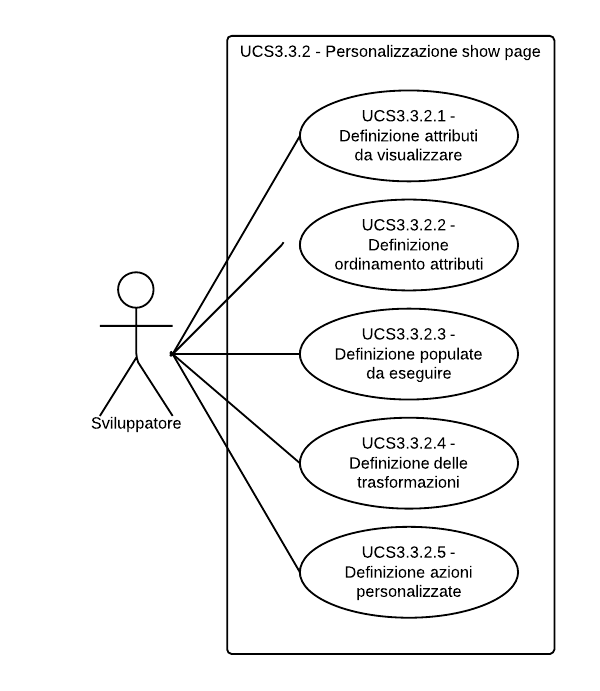
\includegraphics[scale=0.16]{UML/UCS3.3.2 - Personalizzazione show page.png}
      \caption{UCS3.3.2 - Personalizzazione show page} 
    \end{figure}
    \end{center}
    
      %Tabella 
      \begin{center}
      \bgroup
      \def\arraystretch{1.8}     
      \begin{longtable}{  p{3.5cm} | p{8cm} } 
            
      \hline
      \multicolumn{2}{ | c | }{ \cellcolor[gray]{0.9} \textbf{UCS3.3.2 - Personalizzazione show page}} \\ 
      \hline
      
      \textbf{Attori Primari} & Sviluppatore \\ 
          \textbf{Scopo e Descrizione} & Lo sviluppatore personalizza la show page della Collection selezionata. \\ 
          
          \textbf{Precondizioni}  & Il Framework MaaP è funzionante e la Collection da configurare è stata registrata.\\ 
          
          \textbf{Postcondizioni} & Il Framework MaaP ha configurato correttamente la show page della Collection. \\
          
          \textbf{Flusso Principale} & 1. Lo sviluppatore definisce gli attributi da visualizzare nella show page (UCS3.3.2.1);
2. Lo sviluppatore definisce l'ordinamento degli attributi nella show page (UCS3.3.2.2);
3. Lo sviluppatore definisce attributi che contengono attributi innestati o array di attributi (UCS3.3.2.3);
4. Lo sviluppatore definisce delle trasformazioni sugli attributi (UCS3.3.2.4);
5. Lo sviluppatore definisce delle azioni personalizzate da eseguire all'interno della show page (UCS3.3.2.5). \\
          
      \end{longtable}
      \egroup
\end{center}

\subsubsection{UCS3.3.2.1 - Definizione attributi da visualizzare} 
      %Tabella 
      \begin{center}
      \bgroup
      \def\arraystretch{1.8}     
      \begin{longtable}{  p{3.5cm} | p{8cm} } 
            
      \hline
      \multicolumn{2}{ | c | }{ \cellcolor[gray]{0.9} \textbf{UCS3.3.2.1 - Definizione attributi da visualizzare}} \\ 
      \hline
      
      \textbf{Attori Primari} & Sviluppatore \\ 
          \textbf{Scopo e Descrizione} & Lo sviluppatore all'interno del file di configurazione della Collection specifica quali attributi visualizzare nella show page. \\ 
          
          \textbf{Precondizioni}  & Il Framework MaaP è funzionante e la Collection è registrata.\\ 
          
          \textbf{Postcondizioni} & Il Framework MaaP ha apportato le modifiche alla configurazione della Collection. \\
          
          \textbf{Flusso Principale} &  \\
          
      \end{longtable}
      \egroup
\end{center}

\subsubsection{UCS3.3.2.2 - Definizione ordinamento attributi} 
      %Tabella 
      \begin{center}
      \bgroup
      \def\arraystretch{1.8}     
      \begin{longtable}{  p{3.5cm} | p{8cm} } 
            
      \hline
      \multicolumn{2}{ | c | }{ \cellcolor[gray]{0.9} \textbf{UCS3.3.2.2 - Definizione ordinamento attributi}} \\ 
      \hline
      
      \textbf{Attori Primari} & Sviluppatore \\ 
          \textbf{Scopo e Descrizione} & Lo sviluppatore all'interno del file di configurazione della Collection specifica l'ordinamento degli attributi da visualizzare nella show page. \\ 
          
          \textbf{Precondizioni}  & Il Framework MaaP è funzionante e la Collection è registrata.\\ 
          
          \textbf{Postcondizioni} & Il Framework MaaP ha apportato le modifiche alla configurazione della Collection. \\
          
          \textbf{Flusso Principale} &  \\
          
      \end{longtable}
      \egroup
\end{center}

\subsubsection{UCS3.3.2.3 - Definizione populate da eseguire} 
      %Tabella 
      \begin{center}
      \bgroup
      \def\arraystretch{1.8}     
      \begin{longtable}{  p{3.5cm} | p{8cm} } 
            
      \hline
      \multicolumn{2}{ | c | }{ \cellcolor[gray]{0.9} \textbf{UCS3.3.2.3 - Definizione populate da eseguire}} \\ 
      \hline
      
      \textbf{Attori Primari} & Sviluppatore \\ 
          \textbf{Scopo e Descrizione} & Lo sviluppatore all'interno del file di configurazione della Collection specifica attributi che contengono attributi innestati o un array di Document tramite la funzione populate. \\ 
          
          \textbf{Precondizioni}  & Il Framework MaaP è funzionante e la Collection è registrata.\\ 
          
          \textbf{Postcondizioni} & Il Framework MaaP ha apportato le modifiche alla configurazione della Collection. \\
          
          \textbf{Flusso Principale} &  \\
          
      \end{longtable}
      \egroup
\end{center}

\subsubsection{UCS3.3.2.4 - Definizione delle trasformazioni} 
      %Tabella 
      \begin{center}
      \bgroup
      \def\arraystretch{1.8}     
      \begin{longtable}{  p{3.5cm} | p{8cm} } 
            
      \hline
      \multicolumn{2}{ | c | }{ \cellcolor[gray]{0.9} \textbf{UCS3.3.2.4 - Definizione delle trasformazioni}} \\ 
      \hline
      
      \textbf{Attori Primari} & Sviluppatore \\ 
          \textbf{Scopo e Descrizione} & Lo sviluppatore all'interno del file di configurazione della Collection specifica delle trasformazioni sui valori degli attributi che visualizzeranno l'attributo in base all'output della funzione di trasformazione. \\ 
          
          \textbf{Precondizioni}  & Il Framework MaaP è funzionante e la Collection è registrata.\\ 
          
          \textbf{Postcondizioni} & Il Framework MaaP ha apportato le modifiche alla configurazione della Collection. \\
          
          \textbf{Flusso Principale} &  \\
          
      \end{longtable}
      \egroup
\end{center}

\subsubsection{UCS3.3.2.5 - Definizione azioni personalizzate} 
      %Tabella 
      \begin{center}
      \bgroup
      \def\arraystretch{1.8}     
      \begin{longtable}{  p{3.5cm} | p{8cm} } 
            
      \hline
      \multicolumn{2}{ | c | }{ \cellcolor[gray]{0.9} \textbf{UCS3.3.2.5 - Definizione azioni personalizzate}} \\ 
      \hline
      
      \textbf{Attori Primari} & Sviluppatore \\ 
          \textbf{Scopo e Descrizione} & Lo sviluppatore all'interno del file di configurazione della Collection definisce delle azioni personalizzate che potranno essere eseguite dalla show page. Deve essere possibile specificare dei permessi per l'esecuzione di ciascuna azione personalizzata, in caso venga omessa chiunque potrà eseguirla. \\ 
          
          \textbf{Precondizioni}  & Il Framework MaaP è funzionante e la Collection è registrata.\\ 
          
          \textbf{Postcondizioni} & Il Framework MaaP ha apportato le modifiche alla configurazione della Collection. \\
          
          \textbf{Flusso Principale} &  \\
          
      \end{longtable}
      \egroup
\end{center}

\subsubsection{UCS3.3.3 - Rinominazione Collection} 
      %Tabella 
      \begin{center}
      \bgroup
      \def\arraystretch{1.8}     
      \begin{longtable}{  p{3.5cm} | p{8cm} } 
            
      \hline
      \multicolumn{2}{ | c | }{ \cellcolor[gray]{0.9} \textbf{UCS3.3.3 - Rinominazione Collection}} \\ 
      \hline
      
      \textbf{Attori Primari} & Sviluppatore \\ 
          \textbf{Scopo e Descrizione} & Lo sviluppatore può rinominare una collection creata. \\ 
          
          \textbf{Precondizioni}  & Il Framework è funzionante e la Collection da configurare è stata registrata e lo sviluppatore intende rinominarla.Il Framework \\ 
          
          \textbf{Postcondizioni} & Il Framework attraverso le informazioni date dallo sviluppatore ha rinominato la Collection desiderata. \\
          
          \textbf{Flusso Principale} &  \\
          
      \end{longtable}
      \egroup
\end{center}

\subsubsection{UCS3.3.4 - Definizione ordinamento Collection} 
      %Tabella 
      \begin{center}
      \bgroup
      \def\arraystretch{1.8}     
      \begin{longtable}{  p{3.5cm} | p{8cm} } 
            
      \hline
      \multicolumn{2}{ | c | }{ \cellcolor[gray]{0.9} \textbf{UCS3.3.4 - Definizione ordinamento Collection}} \\ 
      \hline
      
      \textbf{Attori Primari} & Sviluppatore \\ 
          \textbf{Scopo e Descrizione} & Lo sviluppatore può definire l'ordinamento della collection rispetto alle altre collection già registrate. \\ 
          
          \textbf{Precondizioni}  & Il Framework è funzionante e la Collection di cui definire l'ordinamento è stata registrata.\\ 
          
          \textbf{Postcondizioni} & Il Framework ha appreso le informazioni date dallo sviluppatore e ha definito l'ordinamento della Collection. \\
          
          \textbf{Flusso Principale} &  \\
          
      \end{longtable}
      \egroup
\end{center}

\subsubsection{UCS3.4 - Registrazione automatica Collection} 
      %Tabella 
      \begin{center}
      \bgroup
      \def\arraystretch{1.8}     
      \begin{longtable}{  p{3.5cm} | p{8cm} } 
            
      \hline
      \multicolumn{2}{ | c | }{ \cellcolor[gray]{0.9} \textbf{UCS3.4 - Registrazione automatica Collection}} \\ 
      \hline
      
      \textbf{Attori Primari} & Sviluppatore \\ 
          \textbf{Scopo e Descrizione} & Lo sviluppatore crea automaticamente una nuova Collection da linea di comando. \\ 
          
          \textbf{Precondizioni}  & Il Framework MaaP è funzionante e lo sviluppatore ha creato un progetto.\\ 
          
          \textbf{Postcondizioni} & Il Framework MaaP ha registrato correttamente la nuova Collection. \\
          
          \textbf{Flusso Principale} &  \\
          
      \end{longtable}
      \egroup
\end{center}

\subsubsection{UCS3.5 - Definizione namespace} 
      %Tabella 
      \begin{center}
      \bgroup
      \def\arraystretch{1.8}     
      \begin{longtable}{  p{3.5cm} | p{8cm} } 
            
      \hline
      \multicolumn{2}{ | c | }{ \cellcolor[gray]{0.9} \textbf{UCS3.5 - Definizione namespace}} \\ 
      \hline
      
      \textbf{Attori Primari} & Sviluppatore \\ 
          \textbf{Scopo e Descrizione} & Lo sviluppatore, se la funzione di namespace è abilitata, può definire un namespace per l'applicazione MaaP generata ed associarlo alle Collection da creare. \\ 
          
          \textbf{Precondizioni}  & Il framework MaaP ha generato un'applicazione funzionante.\\ 
          
          \textbf{Postcondizioni} & Il framework MaaP ha un namespace definito al suo interno. \\
          
          \textbf{Flusso Principale} &  \\
          
      \end{longtable}
      \egroup
\end{center}

\subsubsection{UCS4 - Abilitazione namespace} 
      %Tabella 
      \begin{center}
      \bgroup
      \def\arraystretch{1.8}     
      \begin{longtable}{  p{3.5cm} | p{8cm} } 
            
      \hline
      \multicolumn{2}{ | c | }{ \cellcolor[gray]{0.9} \textbf{UCS4 - Abilitazione namespace}} \\ 
      \hline
      
      \textbf{Attori Primari} & Sviluppatore \\ 
          \textbf{Scopo e Descrizione} & L'attore sviluppatore può scegliere se far utilizzare i namespace all'applicazione MaaP. Il namespace viene utilizzato da MaaP per sapere quali file considerare quando gli viene richiesta una pagina. \\ 
          
          \textbf{Precondizioni}  & L'applicazione MaaP è stata creata ed è funzionante.\\ 
          
          \textbf{Postcondizioni} & L'applicazione MaaP dispone delle funzionalità di namespace. \\
          
          \textbf{Flusso Principale} &  \\
          
      \end{longtable}
      \egroup
\end{center}
\subsection{Ambito Utente MaaS}
\subsubsection{UCM - Operazioni ad alto livello} 
    \begin{center}
    \begin{figure}[H]
      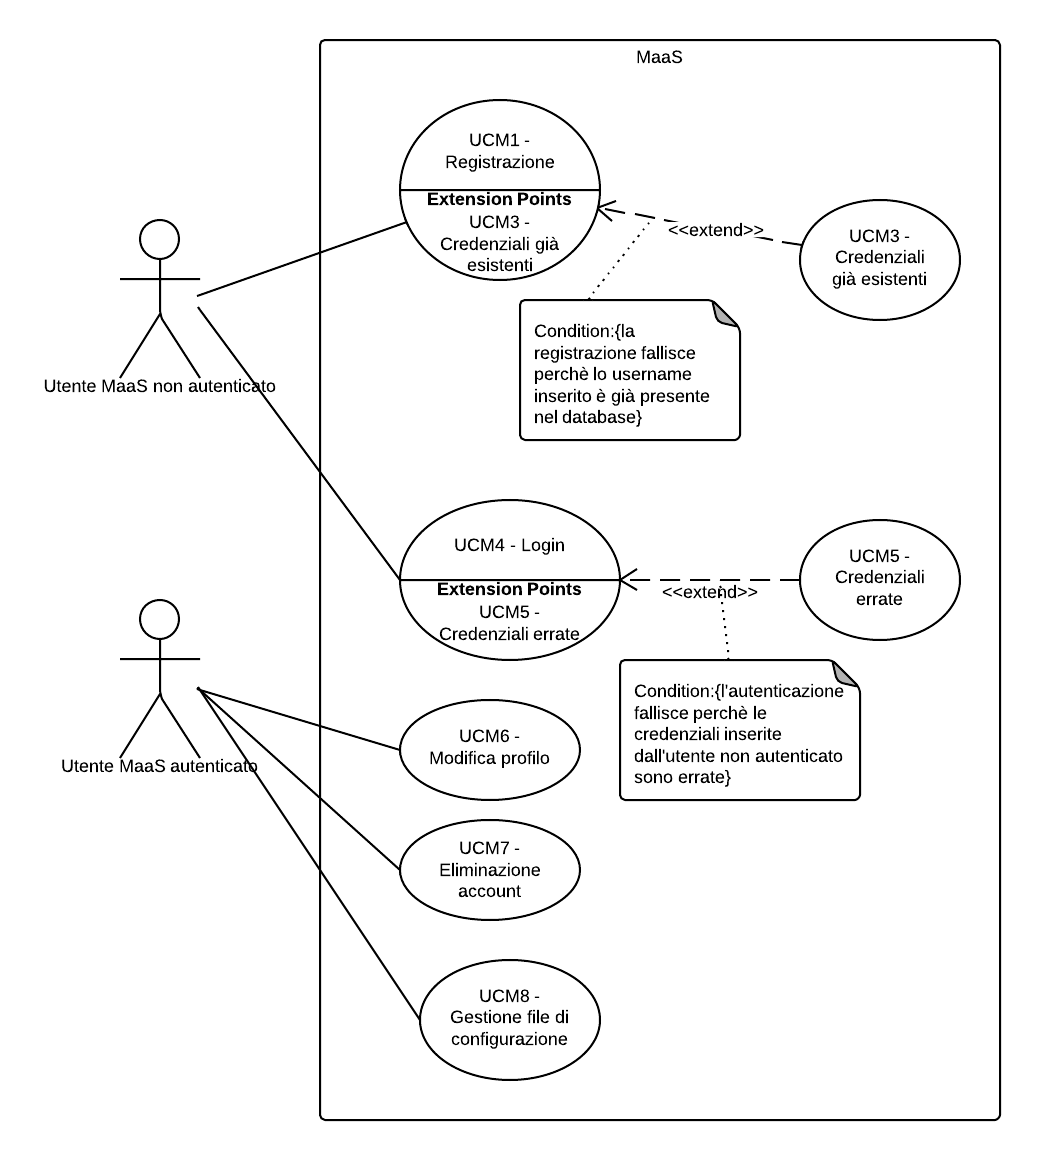
\includegraphics[scale=0.16]{UML/UCM - Operazioni ad alto livello.png}
      \caption{UCM - Operazioni ad alto livello} 
    \end{figure}
    \end{center}
    
      %Tabella 
      \begin{center}
      \bgroup
      \def\arraystretch{1.8}     
      \begin{longtable}{  p{3.5cm} | p{8cm} } 
            
      \hline
      \multicolumn{2}{ | c | }{ \cellcolor[gray]{0.9} \textbf{UCM - Operazioni ad alto livello}} \\ 
      \hline
      
      \textbf{Attori Primari} & Utente MaaS non autenticato, Utente MaaS autenticato \\ 
          \textbf{Scopo e Descrizione} & L'utente MaaS non autenticato può registrarsi al servizio MaaS o effettuare il login.
L'utente MaaS autenticato può modificare il suo profilo, eliminare il proprio account o gestire i file di configurazione per la creazione della pagine. \\ 
          
          \textbf{Precondizioni}  & MaaS è funzionante ed attende che l'utente interagisca.\\ 
          
          \textbf{Postcondizioni} & Il servizio MaaS ha acquisito le informazioni necessarie per svolgere le azioni che l'utente richiede. \\
          
          \textbf{Flusso Principale} & 1. L'utente MaaS non autenticato può registrarsi al servizio (UCM1);
2. L'utente MaaS non autenticato può effettuare il login (UCM4);
3. L'utente MaaS autenticato può modificare il proprio profilo (UCM6);
4. L'utente MaaS autenticato può eliminare il proprio account (UCM7);
5. L'utente MaaS autenticato può gestire i file di configurazione (UCM8). \\
           \textbf{Esclusioni} & 1.1. L'utente visualizza un messaggio di errore dato dall'esistenza delle credenziali inserite per la registrazione (UCM3);
2.1. L'utente visualizza un messaggio di errore dato dall'inserimento in fase di login di credenziali errate (UCU5); \\
      \end{longtable}
      \egroup
\end{center}

\subsubsection{UCM1 - Registrazione} 
      %Tabella 
      \begin{center}
      \bgroup
      \def\arraystretch{1.8}     
      \begin{longtable}{  p{3.5cm} | p{8cm} } 
            
      \hline
      \multicolumn{2}{ | c | }{ \cellcolor[gray]{0.9} \textbf{UCM1 - Registrazione}} \\ 
      \hline
      
      \textbf{Attori Primari} & Utente MaaS non autenticato \\ 
          \textbf{Scopo e Descrizione} & L'utente MaaS non autenticato intende registrarsi al servizio. \\ 
          
          \textbf{Precondizioni}  & MaaS è pronto all'utilizzo.\\ 
          
          \textbf{Postcondizioni} & Il sistema MaaS ha registrato correttamente l'utente e assegnatogli il namespace.
 \\
          
          \textbf{Flusso Principale} &  \\
          
      \end{longtable}
      \egroup
\end{center}

\subsubsection{UCM1.1 - Inserimento nuova email} 
      %Tabella 
      \begin{center}
      \bgroup
      \def\arraystretch{1.8}     
      \begin{longtable}{  p{3.5cm} | p{8cm} } 
            
      \hline
      \multicolumn{2}{ | c | }{ \cellcolor[gray]{0.9} \textbf{UCM1.1 - Inserimento nuova email}} \\ 
      \hline
      
      \textbf{Attori Primari} & Utente MaaS non autenticato \\ 
          \textbf{Scopo e Descrizione} & L'utente inserisce la nuova email nell'intento di registrarsi. \\ 
          
          \textbf{Precondizioni}  & Il servizio visualizza la pagina di registrazione per l'utente che l'ha richiesta ed è in attesa che l'utente interagisca.\\ 
          
          \textbf{Postcondizioni} & MaaP ha appreso le informazioni inserite dall'utente. \\
          
          \textbf{Flusso Principale} &  \\
          
      \end{longtable}
      \egroup
\end{center}

\subsubsection{UCM1.2 - Inserimento nuova password} 
      %Tabella 
      \begin{center}
      \bgroup
      \def\arraystretch{1.8}     
      \begin{longtable}{  p{3.5cm} | p{8cm} } 
            
      \hline
      \multicolumn{2}{ | c | }{ \cellcolor[gray]{0.9} \textbf{UCM1.2 - Inserimento nuova password}} \\ 
      \hline
      
      \textbf{Attori Primari} & Utente MaaS autenticato \\ 
          \textbf{Scopo e Descrizione} & L'utente desidera inserire la password con la quale creerà un account presso il servizio MaaS. \\ 
          
          \textbf{Precondizioni}  & Il sistema MaaS visualizza la pagina di registrazione all'utente che intende registrarsi ed è pronta all'interazione.\\ 
          
          \textbf{Postcondizioni} & Il servizio MaaS ha acquisito le informazioni inserite dall'utente. \\
          
          \textbf{Flusso Principale} &  \\
          
      \end{longtable}
      \egroup
\end{center}

\subsubsection{UCM3 - Credenziali già esistenti} 
      %Tabella 
      \begin{center}
      \bgroup
      \def\arraystretch{1.8}     
      \begin{longtable}{  p{3.5cm} | p{8cm} } 
            
      \hline
      \multicolumn{2}{ | c | }{ \cellcolor[gray]{0.9} \textbf{UCM3 - Credenziali già esistenti}} \\ 
      \hline
      
      \textbf{Attori Primari} & Utente MaaS non autenticato \\ 
          \textbf{Scopo e Descrizione} & Il servizio mostra all'utente MaaS non autenticato un messaggio di errore dato dall'esistenza delle credenziali che aveva inserito per registrarsi. \\ 
          
          \textbf{Precondizioni}  & Il servizio ha appreso le informazioni di registrazione inserite dall'utente.\\ 
          
          \textbf{Postcondizioni} & il servizio MaaS ha respinto la registrazione da parte dell'utente mostrando un errore. \\
          
          \textbf{Flusso Principale} &  \\
          
      \end{longtable}
      \egroup
\end{center}

\subsubsection{UCM4 - Login} 
      %Tabella 
      \begin{center}
      \bgroup
      \def\arraystretch{1.8}     
      \begin{longtable}{  p{3.5cm} | p{8cm} } 
            
      \hline
      \multicolumn{2}{ | c | }{ \cellcolor[gray]{0.9} \textbf{UCM4 - Login}} \\ 
      \hline
      
      \textbf{Attori Primari} & Utente MaaS non autenticato \\ 
          \textbf{Scopo e Descrizione} & L'utente MaaS non autenticato intende accedere al servizio e per farlo deve inserire le proprie credenziali. \\ 
          
          \textbf{Precondizioni}  & Il servizio MaaS è pronto ed attende il login dell'utente.\\ 
          
          \textbf{Postcondizioni} & Il servizio Maas ha verificato le credenziali utente ed ha eseguito l'autenticazione di quest'ultimo. \\
          
          \textbf{Flusso Principale} &  \\
          
      \end{longtable}
      \egroup
\end{center}

\subsubsection{UCM5 - Credenziali errate} 
      %Tabella 
      \begin{center}
      \bgroup
      \def\arraystretch{1.8}     
      \begin{longtable}{  p{3.5cm} | p{8cm} } 
            
      \hline
      \multicolumn{2}{ | c | }{ \cellcolor[gray]{0.9} \textbf{UCM5 - Credenziali errate}} \\ 
      \hline
      
      \textbf{Attori Primari} & Utente MaaS non Autenticato \\ 
          \textbf{Scopo e Descrizione} & L'utente visualizza un messaggio di errore dato dall'inserimento di credenziali errate. \\ 
          
          \textbf{Precondizioni}  & Il sistema MaaS verifica le credenziali che l'utente ha inserito.\\ 
          
          \textbf{Postcondizioni} & Il sistema MaaS visualizza all'utente un messaggio di errore dopo aver verificato e non accettato le credenziali inserite. \\
          
          \textbf{Flusso Principale} &  \\
          
      \end{longtable}
      \egroup
\end{center}

\subsubsection{UCM6 - Modifica profilo} 
    \begin{center}
    \begin{figure}[H]
      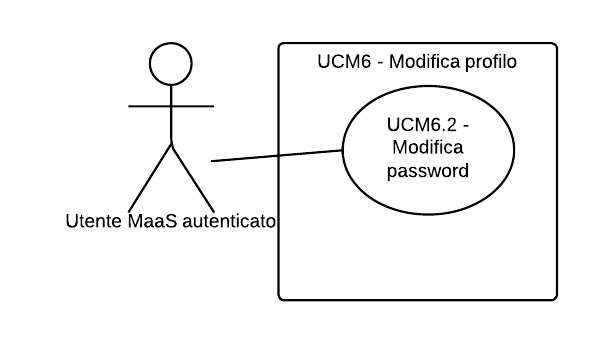
\includegraphics[scale=0.16]{UML/UCM6 - Modifica profilo.png}
      \caption{UCM6 - Modifica profilo} 
    \end{figure}
    \end{center}
    
      %Tabella 
      \begin{center}
      \bgroup
      \def\arraystretch{1.8}     
      \begin{longtable}{  p{3.5cm} | p{8cm} } 
            
      \hline
      \multicolumn{2}{ | c | }{ \cellcolor[gray]{0.9} \textbf{UCM6 - Modifica profilo}} \\ 
      \hline
      
      \textbf{Attori Primari} & Utente MaaS autenticato \\ 
          \textbf{Scopo e Descrizione} & L'utente autenticato nel servizio può modificare i propri dati email e password. \\ 
          
          \textbf{Precondizioni}  & Il sistema è pronto, visualizza la pagina per la modifica del profilo utente e attende che l'utente interagisca.\\ 
          
          \textbf{Postcondizioni} & Il sistema MaaS ha acquisito le informazioni inserite dall'utente ed ha effettuato le modifiche. \\
          
          \textbf{Flusso Principale} & 1. L'utente MaaS autenticato può modificare la propria email (UCU6.1);
2. L'utente MaaS autenticato può modificare la password (UCU6.2). \\
           \textbf{Scenari Alternativi} & L'utente può non modificare i propri dati lasciandoli invariati uscendo dalla pagina. \\
      \end{longtable}
      \egroup
\end{center}

\subsubsection{UCM6.1 - Modifica email} 
      %Tabella 
      \begin{center}
      \bgroup
      \def\arraystretch{1.8}     
      \begin{longtable}{  p{3.5cm} | p{8cm} } 
            
      \hline
      \multicolumn{2}{ | c | }{ \cellcolor[gray]{0.9} \textbf{UCM6.1 - Modifica email}} \\ 
      \hline
      
      \textbf{Attori Primari} & Utente MaaS autenticato \\ 
          \textbf{Scopo e Descrizione} & L'utente intende modificare L'Email. \\ 
          
          \textbf{Precondizioni}  & Il sistema MaaS predispone la pagina di modifica profilo ed attente le modifiche dell'utente.\\ 
          
          \textbf{Postcondizioni} & Il sistema ha acquisito le informazioni date dall'utente. \\
          
          \textbf{Flusso Principale} &  \\
          
      \end{longtable}
      \egroup
\end{center}

\subsubsection{UCM6.2 - Modifica password} 
      %Tabella 
      \begin{center}
      \bgroup
      \def\arraystretch{1.8}     
      \begin{longtable}{  p{3.5cm} | p{8cm} } 
            
      \hline
      \multicolumn{2}{ | c | }{ \cellcolor[gray]{0.9} \textbf{UCM6.2 - Modifica password}} \\ 
      \hline
      
      \textbf{Attori Primari} & Utente MaaS autenticato \\ 
          \textbf{Scopo e Descrizione} & L'utente intende modificare la password di accesso al servizio. \\ 
          
          \textbf{Precondizioni}  & Il sistema predispone della pagina di modifica profilo ed attende che l'utente modifichi la password.\\ 
          
          \textbf{Postcondizioni} & MaaS ha memorizzato l'informazione datagli dall'utente. \\
          
          \textbf{Flusso Principale} &  \\
          
      \end{longtable}
      \egroup
\end{center}

\subsubsection{UCM7 - Eliminazione account} 
      %Tabella 
      \begin{center}
      \bgroup
      \def\arraystretch{1.8}     
      \begin{longtable}{  p{3.5cm} | p{8cm} } 
            
      \hline
      \multicolumn{2}{ | c | }{ \cellcolor[gray]{0.9} \textbf{UCM7 - Eliminazione account}} \\ 
      \hline
      
      \textbf{Attori Primari} & Utente MaaS Autenticato \\ 
          \textbf{Scopo e Descrizione} & L'utente accede alla propria pagina profilo nella quale è presente un azione che gli permette di eliminare il suo account. \\ 
          
          \textbf{Precondizioni}  & Il sistema MaaS ha predisposto una apposita azione per eliminare l'account dell'utente.\\ 
          
          \textbf{Postcondizioni} & Il sistema MaaS ha eliminato l'account dell'utente. \\
          
          \textbf{Flusso Principale} &  \\
          
      \end{longtable}
      \egroup
\end{center}

\subsubsection{UCM8 - Gestione file di configurazione} 
      %Tabella 
      \begin{center}
      \bgroup
      \def\arraystretch{1.8}     
      \begin{longtable}{  p{3.5cm} | p{8cm} } 
            
      \hline
      \multicolumn{2}{ | c | }{ \cellcolor[gray]{0.9} \textbf{UCM8 - Gestione file di configurazione}} \\ 
      \hline
      
      \textbf{Attori Primari} & Utente MaaS Autenticato \\ 
          \textbf{Scopo e Descrizione} & L'utente può gestire i file di configurazione attraverso i quali può registrare una nuova Collection e specificare la connessione al database delle Collection e/o al database delle credenziali. \\ 
          
          \textbf{Precondizioni}  & Il sistema MaaS visualizza la pagina necessaria alla gestione dei file di configurazione.\\ 
          
          \textbf{Postcondizioni} & Il sistema MaaS ha eseguito le azioni di configurazione dell'utente. \\
          
          \textbf{Flusso Principale} &  \\
          
      \end{longtable}
      \egroup
\end{center}

\subsubsection{UCM8.1 - Creazione file di configurazione} 
      %Tabella 
      \begin{center}
      \bgroup
      \def\arraystretch{1.8}     
      \begin{longtable}{  p{3.5cm} | p{8cm} } 
            
      \hline
      \multicolumn{2}{ | c | }{ \cellcolor[gray]{0.9} \textbf{UCM8.1 - Creazione file di configurazione}} \\ 
      \hline
      
      \textbf{Attori Primari} & Utente MaaS Autenticato \\ 
          \textbf{Scopo e Descrizione} & L'utente ha la possibilità di creare il file di configurazione tramite editor di testo o di caricarlo tramite upload. \\ 
          
          \textbf{Precondizioni}  & Il sistema MaaS visualizza la pagina necessaria alla creazione o all'upload dei file di configurazione.\\ 
          
          \textbf{Postcondizioni} & Il sistema MaaS ha eseguito correttamente la creazione del file di configurazione. \\
          
          \textbf{Flusso Principale} & 1. L'utente crea il file di configurazione.
2.L'utente carica il file di configurazione. \\
          
      \end{longtable}
      \egroup
\end{center}

\subsubsection{UCM8.2 - Creazione file di configurazione tramite editor di testo.} 
      %Tabella 
      \begin{center}
      \bgroup
      \def\arraystretch{1.8}     
      \begin{longtable}{  p{3.5cm} | p{8cm} } 
            
      \hline
      \multicolumn{2}{ | c | }{ \cellcolor[gray]{0.9} \textbf{UCM8.2 - Creazione file di configurazione tramite editor di testo.}} \\ 
      \hline
      
      \textbf{Attori Primari} & Utente MaaS Autenticato \\ 
          \textbf{Scopo e Descrizione} & L'utente visualizza un editor di testo con il quale può effettuare la creazione dei file di configurazione. \\ 
          
          \textbf{Precondizioni}  & Il sistema MaaP fornisce un editor di testo per la creazione dei file di configurazione.\\ 
          
          \textbf{Postcondizioni} & Il sistema MaaP fornisce un editor di testo per la creazione dei file di configurazione. \\
          
          \textbf{Flusso Principale} & 1. L'utente crea il file di configurazione \\
          
      \end{longtable}
      \egroup
\end{center}

\subsubsection{UCM8.3 - Creazione file di configurazione tramite caricamento} 
      %Tabella 
      \begin{center}
      \bgroup
      \def\arraystretch{1.8}     
      \begin{longtable}{  p{3.5cm} | p{8cm} } 
            
      \hline
      \multicolumn{2}{ | c | }{ \cellcolor[gray]{0.9} \textbf{UCM8.3 - Creazione file di configurazione tramite caricamento}} \\ 
      \hline
      
      \textbf{Attori Primari} & Utente MaaS Autenticato \\ 
          \textbf{Scopo e Descrizione} & L'utente può caricare il proprio file di configurazione. \\ 
          
          \textbf{Precondizioni}  & Il sistema MaaP fornisce un sistema di caricamento per i file di configurazione.\\ 
          
          \textbf{Postcondizioni} & Il sistema MaaS carica correttamente il file di configurazione \\
          
          \textbf{Flusso Principale} & 1. L'utente carica il proprio file di configurazione. \\
          
      \end{longtable}
      \egroup
\end{center}

\subsubsection{UCM8.4 - Modifica file di configurazione} 
      %Tabella 
      \begin{center}
      \bgroup
      \def\arraystretch{1.8}     
      \begin{longtable}{  p{3.5cm} | p{8cm} } 
            
      \hline
      \multicolumn{2}{ | c | }{ \cellcolor[gray]{0.9} \textbf{UCM8.4 - Modifica file di configurazione}} \\ 
      \hline
      
      \textbf{Attori Primari} & Utente MaaS Autenticato \\ 
          \textbf{Scopo e Descrizione} & L'utente dopo aver scelto il file di configurazione può modificarlo tramite editor di testo. \\ 
          
          \textbf{Precondizioni}  & Il sistema MaaP visualizza il file scelto dall'utente ed è pronto per la modifica.\\ 
          
          \textbf{Postcondizioni} & Il sistema MaaP esegue correttamente la modifica del file e lo salva. \\
          
          \textbf{Flusso Principale} & 1. L'utente tramite editor di testo modifica il file scelto. \\
          
      \end{longtable}
      \egroup
\end{center}

\subsubsection{UCM8.5 - Eliminazione file di configurazione} 
      %Tabella 
      \begin{center}
      \bgroup
      \def\arraystretch{1.8}     
      \begin{longtable}{  p{3.5cm} | p{8cm} } 
            
      \hline
      \multicolumn{2}{ | c | }{ \cellcolor[gray]{0.9} \textbf{UCM8.5 - Eliminazione file di configurazione}} \\ 
      \hline
      
      \textbf{Attori Primari} & Utente MaaS Autenticato \\ 
          \textbf{Scopo e Descrizione} & L'utente può eliminare il file di configurazione scelto. \\ 
          
          \textbf{Precondizioni}  & Il sistema MaaS ha predisposto per ogni file di configurazione la possibilità di eliminarlo.\\ 
          
          \textbf{Postcondizioni} & Il sistema MaaS ha eliminato correttamente il file di configurazione. \\
          
          \textbf{Flusso Principale} & 1. L'utente elimina il file di configurazione \\
          
      \end{longtable}
      \egroup
\end{center}
